\documentclass[10pt,a4paper,oneside]{scrartcl}

% packages
\usepackage{scrhack}
\usepackage{fullpage}
\usepackage{graphicx}
\usepackage[style=numeric,backend=bibtex8,urldate=iso8601]{biblatex}
\usepackage{listings}
\usepackage{courier}
\usepackage{array}
\usepackage{tabularx}
\usepackage{amsmath}
\usepackage{longtable}
\usepackage[iso]{datetime}
\usepackage{pdfpages}

% basic latex configuration
\setlength{\parskip}{\baselineskip}
\setlength{\parindent}{0pt}

% biblatex
\addbibresource{references.bib}

% graphics
\graphicspath{ {./images/} }

% language listings
\lstdefinelanguage{CL}[ANSI]{C}
{
	morekeywords={__kernel,kernel,__local,local,__global,global,__constant,constant,__private,private},
	morekeywords={char2,char3,char4,char8,char16,uchar2,uchar3,uchar4,uchar8,uchar16,short2,short3,short4,short8,short16,ushort2,ushort3,ushort4,ushort8,ushort16,int2,int3,int4,int8,int16,uint2,uint3,uint4,uint8,uint16,long2,long3,long4,long8,long16,ulong2,ulong3,ulong4,ulong8,ulong16,float2,float3,float4,float8,float16,image2d_t,image3d_t,sampler_t,event_t,bool2,bool3,bool4,bool8,bool16,half2,half3,half4,half8,half16,quad,quad2,quad3,quad4,quad8,quad16,complex,imaginary},
	morekeywords={convert_char2,convert_char4,convert_char8,convert_char16,convert_uchar,convert_uchar2,convert_uchar4,convert_uchar8,convert_uchar16,convert_short,convert_short2,convert_short4,convert_short8,convert_short16,convert_ushort,convert_ushort2,convert_ushort4,convert_ushort8,convert_ushort16,convert_int,convert_int2,convert_int4,convert_int8,convert_int16,convert_uint,convert_uint2,convert_uint4,convert_uint8,convert_uint16,convert_long,convert_long2,convert_long4,convert_long8,convert_long16,convert_ulong,convert_ulong2,convert_ulong4,convert_ulong8,convert_ulong16,convert_float,convert_float2,convert_float4,convert_float8,convert_float16}
	morekeywords={write_imagef,write_imagei,write_imageui,read_imagef,read_imagei,read_imageh,read_imageui,get_image_width,get_image_height,get_image_depth,get_image_channel_data_type,get_image_channel_order,get_image_dim,get_work_dim,get_global_size,get_global_id,get_local_size,get_local_id,get_num_groups,get_group_id,cross,dot,distance,length,normalize,fast_distance,fast_normalize,isequal,isnotequal,isgreater,isgreat,erequal,isless,islessequal,islessgreater,isfinite,isinf,isnan,isnormal,isordered,isunordered,signbit,any,bitselect,select,async_work_group_copy,wait_group_events,prefetch,barrier,mem_fence,read_mem_fence,write_mem_fence,acos,acosh,acospi,asin,asinh,asinpi,atan,atan2,atanh,atanpi,atan2pi,cbrt,ceil,copysign,cos,cosh,cospi,erfc,erf,exp,exp2,exp10,expm1,fabs,fdim,floor,fma,fmax,fmin,fmod,fract,floor,frexp,hypot,ilogb,ldexp,lgamma,lgamma_r,log,log2,log10,log1p,logb,mad,modf,nan,nextafter,pow,pown,powr,remainder,remquo,rint,rootn,round,rsqrt,sin,sincos,sinh,sinpi,sqrt,tan,tanh,tanpi,tgamma,trunc,half_cos,half_divide,half_exp,half_exp2,half_exp10,half_log,half_log2,half_log10,half_powr,half_recip,half_rsqrt,half_sin,half_sqrt,half_tan,native_cos,native_divide,native_exp,native_exp2,native_exp10,native_log,native_log2,native_log10,native_powr,native_recip,native_rsqrt,native_sin,native_sqrt,native_tan,mad24,mul24,mul_hi,sub_sat,rotate,mad_sat,clz,rhadd,hadd,add_sat,abs_diff,abs,max,min,upsample,get_global_offset,minmag,maxmag,clamp,async_work_group_strided_copy,vec_step,shuffle,shuffle2}
	sensitive=true,
	morecomment=[l]{//},
	morecomment=[s]{/*}{*/},
	morestring=[b]",
}

\lstset
{
	tabsize=2,
	captionpos=b,
	basicstyle=\ttfamily{},
	aboveskip=\parskip,
% keywordstyle=\color{blue}\bfseries,
% commentstyle=\color{commentgreen},
% stringstyle=\color{red},
	showstringspaces=false,
	breaklines=true,
	numbers=left,
	frame=single,
% backgroundcolor=\color{lightgray}
}

\title{GPGPU Computing with OpenCL}
\subtitle{Comparing GPU accelerated standard algorithms with traditonal CPU implementations}
\author{Bernhard Manfred Gruber}
\date{\today}

\begin{document}


\includepdf{titlepage}
%\maketitle
%\thispagestyle{empty}
%\clearpage

\pagenumbering{Roman}

\section*{Declaration}

I hereby declare and confirm that this thesis is entirely the result of my own original work. Where other sources of information have been used, they have been indicated as such and properly acknowledged. I further declare that this or similar work has not been submitted for credit elsewhere.

\vspace{2cm}

\parbox{7cm}{
	\centering
	\rule{6cm}{1pt}\\
	Hagenberg, \today 
}
\hfill
\parbox{7cm}{
	\centering
	\rule{6cm}{1pt}\\
	Bernhard Manfred Gruber
}

%\section*{Acknowledgments}

Herwig Mayr for helping me to get the internship.

Alexander Leutgeb for excellent support.

RISC Software GmbH for providing me with an awesome work station.

Michael Hava for deepening my knowledge about C++11.

\section*{Kurzfassung}

Diese Arbeit stellt eine detaillierte Dokumentation über das Berufspraktikum des Autors bei der RISC Software GmbH dar. Nach einer kurzen Einführung in das Unternehmen sowie das Projekt Enlight werden die Ziele des Praktikums erläutert, welche verschiedene Aspekte der Implementierung eines Raycasters mit OpenCL betreffen, der in den drei Praktikumsmonaten erstellt wurde.

Im Anschluss an die Einführung werden grundlegende Themen sowie Basiswissen behandelt, das in späteren Kapiteln benötigt wird. Dazu gehört ein Grundverständnis über Raycasting, reguläre Gitter als Beschleunigungsstruktur, Raycasting implizit beschriebener Geometrie über boolsche Subtraktion und OpenCL als Technologie für GPU Beschleunigung.

Bevor sich die Arbeit in die eigentliche Implementierung vertieft, wird der zum Praktikumsbeginn bestehende Prototyp detailliert analysiert. Dabei wird vor allem auf fortgeschrittene Algorithmen zur Optimierung des eingesetzten Raycasting Verfahrens eingegangen.

Anschließend fokussiert sich die Arbeit auf verschiedenen OpenCL Programme, deren Ziel es ist GPU beschleunigt Bilder in ähnlicher Qualität wie die existierende Implementierung zu erzeugen. Auf Vorteile und Schwierigkeiten während der Implementierung der OpenCL Programme wird ebenfalls eingegangen.

Die abschließenden Laufzeitvergleiche der funktionierenden OpenCL Raycaster mit der existierenden CPU Implementierung werden noch durch Erfahrungen mit Entwicklungswerkzeugen rund um OpenCL und einer kurzen Diskussion über noch offene Probleme abgerundet.

\pagebreak

\section*{Abstract}

This thesis provides a detailed coverage of the authors internship at RISC Software GmbH. After a short introduction to the company and the Enlight project, the goals of the internship are discussed, which address various aspects of an OpenCL ray caster implementation created during the three months working period.

In succession to the introduction, fundamental topics required in further chapters of the thesis are covered. These include the principle of ray casting, regular grids as acceleration structure, ray casting implicitly described geometry using boolean subtraction and OpenCL as technology for GPU acceleration.

Before the thesis deepens into the actual implementation, the existing prototype at the start of the internship is analyzed in detail. This includes advanced algorithms to optimize the used ray casting approach.

The primary focus then lies on several OpenCL programs with the goal of reproducing the visual output of the existing CPU implementation using GPU acceleration. Advantages and difficulties of developing with OpenCL are encountered during the explanations of the implementations.

The final benchmarks of the working OpenCL ray casters are than rounded off by experiences made with various development tools around OpenCL and a discussion of the still remaining problems.


\tableofcontents

\clearpage

\pagenumbering{arabic}

\section{Introduction}

\subsection{Motivation}

For a long time the speed of algorithms experienced a constant growth through improved processor hardware. Intel co-founder Gordon E. Moore was one of the first persons to describe this trend in 1965. This description is well known by the name Moore's law which initially stated that the number of transistors on an integrated circuit doubles every year \cite{moore_law}. This trend slowed down and Moore had to change the interval to two years a decade later \cite{moore_law_2003}. The most important consequence however has been realized by one of Moore's co-workers at Intel, David House, who predicted that the performance of processors would double every 18 months \cite{moore_law_2003}. As a result, an increase in computing power could be obtained simply by running the same algorithms on newer hardware. As a consequence, hardware dominated the growth of algorithms' performance for a long period of time.

Unfortunately, processing hardware technologies hit a limit at the beginning of the third millennium. Physical bounds, like the size of atoms, prevented a further shrink of integrated circuits which would allow an increase in clock speed. Therefore, processor vendors like Intel and AMD started to place multiple CPUs on a single chip which still lead to an increase in computational power but in a different way than in the last 40 years. This change is sometimes referred to as the multicore crisis \cite{multicore_crisis}. The consequence from a software developer's perspective is that traditional algorithms stopped gaining speed by being run on newer hardware. In fact, improving performance is now up to the programmer, who is responsible for writing concurrent and parallel software that can make full use of the underlying hardware's capabilities. 

But multicores were not the only major hardware change that had an impact on the way software is developed recently. Graphics cards, which were initially intended to offload and accelerate 2d and 3d graphic operations from the CPU to a separate hardware device, started to gain popularity in non graphical areas of programming. A GPUs intense float processing power and parallel nature by design makes it ideal for uses in several areas of science, business and engineering (General Purpose GPU). When used in the right place, a GPU may compute results several magnitudes faster than the CPU \cite{gpu_history}. However, due to the very different hardware architecture the graphics card is still not suitable to efficiently solve the same problems as a CPU does.

Todays software engineers working in performance focused domains have a hard time designing their applications and algorithms. With two very different types of processors (CPU and GPU), both excellent in their own ways, and a lot of APIs and frameworks around them (OpenMP, CUDA, OpenCL, DirectCompute, C++ AMP, ...), the available hardware and software to access it is more heterogeneous than ever. Thus, profound knowledge of the available technologies, their performance and restrictions as well as the consequences for a development team is essential for choosing the optimal strategy to tackle todays computational needs.

\subsection{Goal}
The goal of this thesis is to provide the reader with a state of the art comparison of modern GPU and CPU performance in solving traditional problems such as sorting arrays and multiplying matrices using various approaches.
The GPU algorithms will be implemented using the Open Computing Language (OpenCL). Therefore the reader is given a short introduction into OpenCL in order to understand the provided code samples and how programming for a GPU works. These OpenCL implementations are benchmarked against algorithms implemented in C/C++ solving the same problem. It is important to note that the GPU and CPU version do not necessarily have to use the same algorithm, they only have to output the same result. This decision was inevitable due to the highly diverse hardware properties of the CPU and the GPU.
The problems chosen for this comparison are sorting an array, multiplying two large matrices and calculating the parallel prefix sum of an array (explained in corresponding chapter \ref{sec:prefix_sum}). These algorithms cover several different aspects that play an important role when implementing an algorithm for a GPU such as runtime complexity, memory footprint and memory transfer time vs. computation time. 

Eventually, the results of benchmarking the chosen algorithms should give the reader an idea how much a GPU can accelerate different kinds of algorithms and what a programmer has to pay attention to when developing GPGPU accelerated software. This knowledge is not only valuable during developing but also useful when choosing the right technology for a given problem. This thesis should aid all software engineers in understanding how GPU computing works and where it should be used.

\subsection{History of GPGPU Computing} 
\label{sec:history}
Before we start into details about OpenCL and several GPU implementations, some background information about how GPUs have evolved is provided which may help understanding the design and peculiarities of graphics hardware. The following information is taken from a paper survey in 2010 \cite{gpu_history}.

In the early 1980's a "GPU" was nothing more than an integrated frame buffer, an additional chip that relied on the CPU for drawing.

One of the first dedicated video cards was the IBM Professional Graphics Controller (PGA) released in 1984. It used an on-board Intel 8088 microprocessor to take care of graphical calculations in order to take off load from the main processor. Although the Intel 8088 was in fact a conventional CPU, the PGA's separate on-board processing unit marked an important step towards the development of GPUs as co-processors.

In the following years more graphics orientated features where added like shading, lighting, rasterization, the depth buffer and color blending. With the introduction of OpenGL in 1989 by Silicon Graphics Inc. (SGI), the world's first application programming interface (API) for 2D and 3D graphics was released. OpenGL was designed upon a concept called the graphics pipeline which depicts video processing as data traveling through multiple stages of operations. The pipeline begins at the CPU by sending geometry data together with colors, textures etc., which is then transformed from the initial 3D coordinate space to pixel coordinates. Lighting operations use material colors and textures to shade the incoming triangles which are then rasterized into the frame buffer for display. As the programmer was not able to alter the functionality if the pipeline it is also well known under the term "fixed function pipeline". This processing model determined the design of graphics hardware for more then a decade.

In the mid 1990's NVIDIA, ATI and Matrox started to provide graphic controllers for consumers. Famous computer games like Quake and Doom became popular spurring the gaming industry and the interest in GPUs. However, GPUs at this time were only able to output one pixel per clock cycle and CPUs were able to send more triangles than the GPU could handle. This problem lead graphic hardware vendors to adding more pipelines and eventually more cores to their GPUs in order to enable parallel pixel processing and increase the throughput.

NVIDIA's release of the GeForce 3 in 2001 marked an important step in the evolution of GPUs by loosening the restrictions of the fixed function pipeline. With the ability of writing small programs for the GPU, which could operate on the vertices traveling through the pipeline, programmers were given a tool to make limited changes to the behavior of the pipeline. These programs were called vertex shaders and were written in an assembly-like language. One year later the pixel shader followed running on a separate part of the GPU hardware.

\begin{figure} % from http://wiki.ega.org.pl/images/b/b4/Pipeline.png
\centering
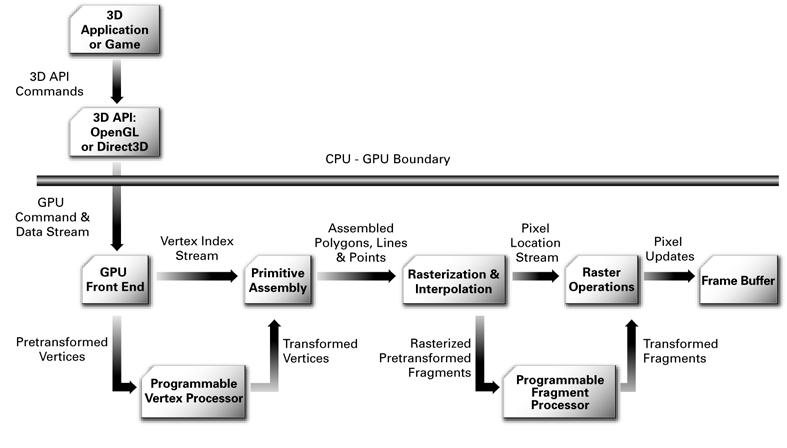
\includegraphics[width=0.7\linewidth]{pipeline2}
\caption{The graphics pipeline with programmable vertex and fragment processor. \cite{cg_book}}
\label{fig:pipeline2}
\end{figure}

With the introduction of the High Level Shading Language (HLSL) with DirectX 9 in 2003 programming GPU hardware became easier than with the previous shaders written in assembler. The first developers started to use the available programmability for non-graphical tasks. The first attempts of GPU computing emerged. A year later in 2004 Brook and Sh appeared representing the first languages targeting GPGPU computing.
Although the workflow of the GPU is still based on a programmable graphics pipeline, the hardware mainly consists of strong, highly parallel floating-point processors with fast memory access.

In 2006 the GeForce 8800 featured the first GPU with a unified programmable processor called a streaming multiprocessor which is used to execute the vertex, pixel and a new geometry shader. The graphics pipeline has become only a software concept used by graphic APIs such as OpenGL and DirectX.

Software GPGPU support was introduced by NVIDIA with the Compute Unified Device Architecture (CUDA). It offers a C like language to create general purpose programs (called kernels) that can be executed on the GPU. ATI followed with the ATI Stream technology and Microsoft introduced compute shaders with DirectX 10.

In 2010 NVIDIA released the first GPU based on their Fermi architecture which was explicitly designed for GPGPU computing. The GTX580 Fermi GPU released later that year contained 16 streaming multiprocessors with 512 CUDA cores and accessed 1.5 GiB GDDR5 RAM with a bandwidth of 192.4 GB/s \cite{gtx580_spec}.

\subsection{Chapter overview}

After this short introduction chapter \ref{sec:opencl} will continue with a comprehensive coverage of OpenCL. Beside general information about the API, this chapter focuses on the knowledge required to understand how OpenCL executes kernels on the GPU and what a developer has to pay attention to when programming for graphics hardware. This information is vital for understanding the implemented algorithms in the subsequent chapters.

Chapter \ref{sec:matrix_mul} will present the first OpenCL implementation of a standard algorithm by tackling multiplications of large floating point matrices. Beside a simply and naive approach, several possibilities of optimizations are discussed introducing graphic hardware features like shared memory, texture memory and vector types.

\pagebreak

Chapter \ref{sec:prefix_sum} continues with implementations of a prefix sum algorithm (also known as scan) - a ridiculous simple problem for a CPU due to its sequential nature. However, the linearity if the algorithm does not fit the architecture of a GPU. A tree based approach is discussed which is commonly used to partly parallelize linear algorithms.

Chapter \ref{sec:sorting} focuses sorting as one of the most famous problems in computer science. Several well performing CPU implementations such as C's qsort and C++'s std::sort will be compared with GPU sorting techniques using less popular algorithms such as the bitonic sorting network and radix sort.


\section{OpenCL}
\label{sec:opencl}

\subsection{What is OpenCL?}
OpenCL is specified by the Khronos Group in the OpenCL 1.2 Specification as follows:

\begin{quote}
OpenCL (Open Computing Language) is an open royalty-free standard for general purpose
parallel programming across CPUs, GPUs and other processors, giving software developers
portable and efficient access to the power of these heterogeneous processing platforms. \cite{opencl_spec}
\end{quote}

The Khronos Group is an industry consortium who maintains OpenCL as an open standard. This means that the Khronos Group offers a specification of the OpenCL API and a detailed description about its functionality and behavior for free. This specification can be downloaded at their website \cite{opencl_spec}. Maintaining the OpenCL standard consequently means, that the Khronos Group neither provides software development kits (SDKs), drivers that implement OpenCL nor hardware that it can make use of. These concerns are subject to other companies called vendors, which are typically hardware manufacturers providing necessary developing resources and include OpenCL support in their drivers. Examples of such companies are the two famous graphic card vendors NVIDIA and AMD as well as the renowned processor manufacturer Intel.

Unlike other famous APIs the Khronos Groups specifies which are very specific in their usage or the targeted hardware (like the famous 3D API OpenGL used to drive graphic hardware), OpenCL is a general purpose programming framework. It was conceived with universality in mind, offering almost no restrictions on the field of application it may be used in. Portability from its well designed hardware abstraction model, which enables it to run on many different kinds of devices, even ones which may have not been created yet, is one of OpenCL most powerful strengths. Such devices may be classical CPUs and GPUs, but also more uncommon types of hardware like FPGAs (field programmable gate arrays), DSPs (digital signal processors) or Intel's MICs (Many Integrated Core) \cite{mic}. Moreover, OpenCL may be used to combine multiple available devices into a single heterogeneous platform extending an applications processing resources beyond the bounds of individual pieces of hardware.

Additionally to being independent of a specific purpose and decoupled from the underlying hardware, OpenCL is also available across all mayor operations systems including Windows, Linux and Mac OS X.

With the upcoming specification of WebCL (currently available as a working draft), OpenCL will eventually even find its way into web browsers and the HTML5 technology. Thus making it even independent of an operating system and bringing high performance computing into web applications.

\subsection{Components}

OpenCL is not an API alone. As it allows programs to run on hardware that may have certain restrictions or offer different features than a classical CPU, traditional languages like C++, Java or C\# can not be used to write those programs. Therefore, the OpenCL standard includes the specification of a separate language that is used to write small programs that are executed on a hardware device. These programs are called kernels and are written in the OpenCL C language, which is a restricted version of C99 with extensions for vectorization and handling OpenCL's abstract memory model.

\pagebreak

To allow OpenCL to support many different hardware platforms it consists of the following components:

\begin{description}
	\item[API] \hfill \\
	The application programming interface is specified by the Khronos Group, ensuring that every vendor implementation of OpenCL is compatible and exchangeable. The API is provided as a set of C header files that a software developer can download from Khronos' website. These headers are typically also shipped within an SDK. Khronos additionally specifies a C++ wrapper around C API. Bindings for other languages exist but they are not maintained by Khronos.
	The API is used by a conventional program (e.g. written in C++) to run kernels on an OpenCL capable device. This program is called the host application.
	\item[SDK] \hfill \\
	The software developing kit is the main collection of tools and resources a software developer needs to write applications using OpenCL. An SDK is usually provided by a vendor, an implementor of OpenCL. Examples of such SDKs are the NVIDIA CUDA Toolkit and AMD's Accelerated Parallel Processing (APP) SDK. These SDKs typically contain header files to be included by a C/C++ program and static libraries for the linker, which are responsible for binding to the OpenCL driver at runtime. Furthermore, code examples, tutorials, documentation, developing tools etc. may be additionally provided depending on the vendor. With headers and static libraries an SDK contains all resources necessary to write and compile an OpenCL application.
	\item[OpenCL C language] \hfill \\
	Kernels are typically written in separate source files using the OpenCL C language. An OpenCL application reads these source files at run time and sends them to the OpenCL compiler to create a binary for one or more available hardware devices where it may be executed. A source file written in the OpenCL C language may consist of several functions, variable definitions, control flow statements, comments, etc., but has to have at least one function prefixed with the \lstinline!__kernel! attribute. This function may be called by the host application through the OpenCL API and serves as an entry point into a kernel.
	\item[OpenCL C Compiler] \hfill \\
	OpenCL kernels must be compiled for a specific platform before they can be executed. This compilation process is initiated and controlled by the host application through the API. The separate compilation at run time is required to retain OpenCL's portability, as an OpenCL application may be deployed on any kind of machine with a suitable driver. Consequently, the available OpenCL implementation (providing the compiler) and the used hardware device (affecting the compiler's output) may only be determined at runtime.
	\item[Driver] \hfill \\
	Finally, the driver is OpenCL's core. It implements the OpenCL API and maps the functionality specified in the standard to a vendor's hardware. The host application uses the driver through the API to initialize OpenCL, compile kernels, allocate memory resources, initiate computations and communicate with kernels running on a device. A driver is always specific to a dedicated hardware and must therefore be provided by a vendor. The driver is sometimes also referred to as Installable Client Driver (ICD).
\end{description}

\subsection{Hardware architectures}
\label{sec:hardware_arch}

One of the greatest advantages of OpenCL and also one of the biggest influences on its design is OpenCL's ability to support devices of many different hardware architectures. These devices can be used through OpenCL by the same common API and may even be used together in a single application or computation, which is sometimes referred to as heterogeneous computing.
A closer look into the architectures of the two most common hardware devices, namely a CPU and a GPU, may aid the reader to better understand design decisions made by the Khronos Group when OpenCL was conceived. Furthermore, a deeper understanding of graphics hardware will be needed for the implementation chapters of this thesis.

\subsubsection{Central Processing Unit (CPU)}

The CPU is the kind of processors developers are mostly used to. Software written in common languages like C++, Java or C\# is directly or indirectly (using a Virtual Machine) executed on this kind of hardware.
In figure \ref{fig:ivy_bridge} we can see the design of a modern processor by the example of an Intel Ivy Bridge quad-core. One can clearly see the four physical cores of the processor. Thanks to hardware multithreading (Hyper-threading in Intel terms) each physical core can process a pair of threads which are seen as two virtual CPUs by the operation system resulting in 8 available cores for an application.
Note the on-chip graphics processor in the Ivy Bridge architecture which can be used as a replacement for a graphics card. It is however not used as general processing device such as the CPU's cores.

\begin{figure}
\centering
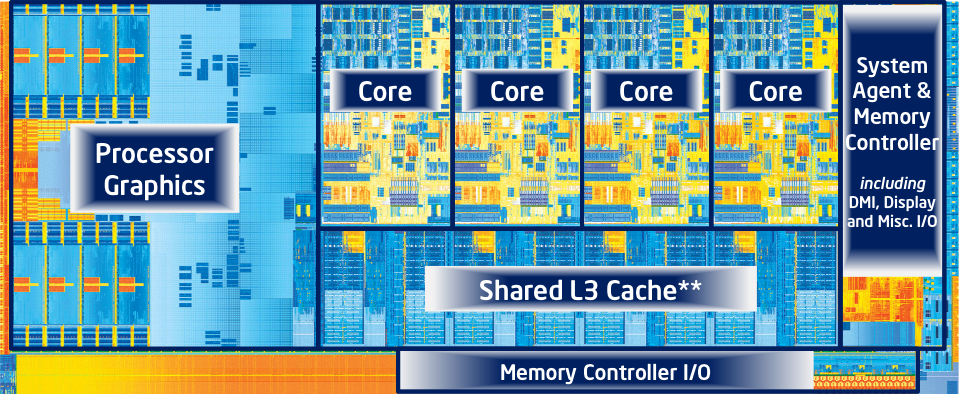
\includegraphics[width=0.9\textwidth]{ivy_bridge}
\caption{Architectural overview of an Intel Ivy Bridge processor. \cite{ivy_bridge}}
\label{fig:ivy_bridge}
\end{figure}

When it comes down to calculative throughput, and the tackled problem offers some degree of data parallelism (several chunks of data are processed equally), SIMD (Single Instruction Multiple Data) features of the CPU can be used to increase the number of input elements an instruction can process. Intel's Ivy Bridge for example allows the parallel execution (vectorization) of up eight single precision floating point operations using AVX (Advanced Vector Extensions, successor of SSE - Streaming SIMD Extensions) instructions.

Considering memory access, the CPU uses the standard data bus to communicate with the external main memory. As this communication usually takes a while (up to hundreds or even thousands of CPU cycles \cite[p.54]{opencl_book}), the CPU uses a hierarchical cache system. Each core has it's own level one and level two cache, which have to be kept synchronized to the other cores. All cores share a common level three cache that is further connected to the memory controller.

From a performance concerned developer's perspective, all we have to pay attention to is to have enough parallelism in our application to utilize all cores of our CPU (which is typically a number of 2, 4 or 8 on consumer hardware). If our application has to process large amounts of data using the same operations on elements of the input (e.g. multimedia applications like image or video processing), vector instructions may be used to speed up execution. Regarding memory, beside small adjustments to improve cache effects the developer has only limited power to optimize, as the entire cache system is controlled by the CPU and operation system. 


\subsubsection{Graphics Processing Unit (GPU)}
\label{sec:gpu}

When we think of a GPU we think of a highly parallel, graphics orientated processing device. From its introduction with OpenGL in 1989 until the creation of the first GPGPU languages in 2004 (cf. chapter \ref{sec:history}), the architecture of a GPU's hardware followed the principles of the graphics pipeline. To fit this purpose, GPUs developed from original desktop processors to (as written in the book Heterogeneous Computing with OpenCL \cite{opencl_book}) heavily multithreaded devices employing sophisticated task management directly in hardware. This was needed to cope with complex task graphs processing vertices, geometry and pixels. This tasks and the data they process are highly parallel and represent an extensive amount of independent work, which is therefore most suitably handled by a device with a great amount of cores employing latency tolerant multithreading\footnote{Latency tolerant processing units are characterized by being insensitive to longer lasting memory requests.}.

\begin{figure}
\centering
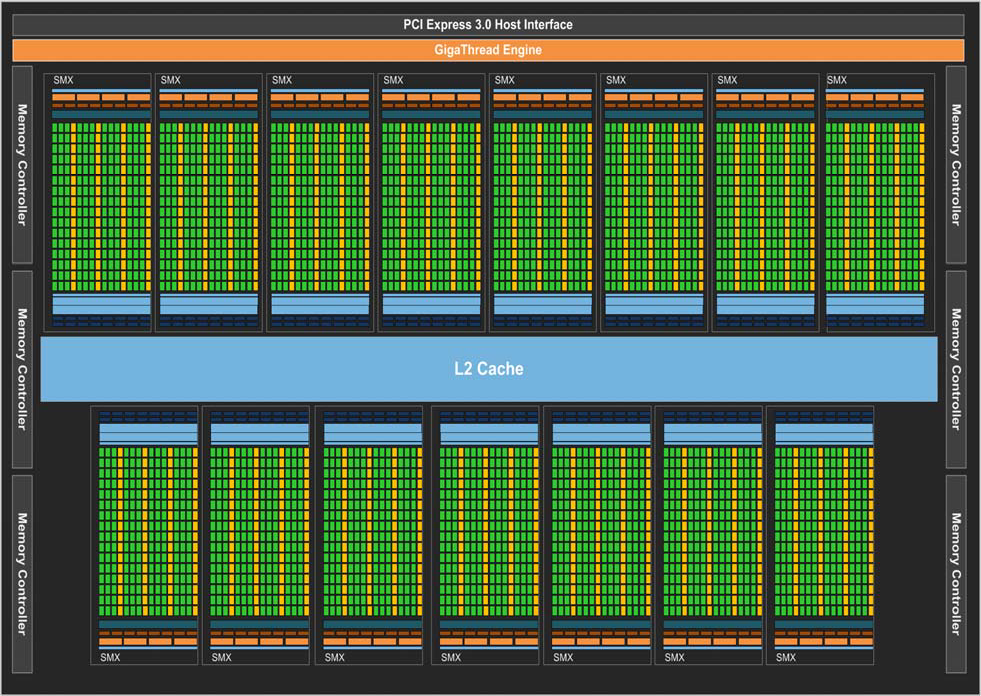
\includegraphics[width=0.9\textwidth]{kepler_arch}
\caption{Full chip block diagram of NVIDIA's Kepler GK110 architecture containing 15 streaming multiprocessors (SMX). \cite{kepler_arch}}
\label{fig:kepler_arch}
\end{figure}

\begin{figure}
\centering
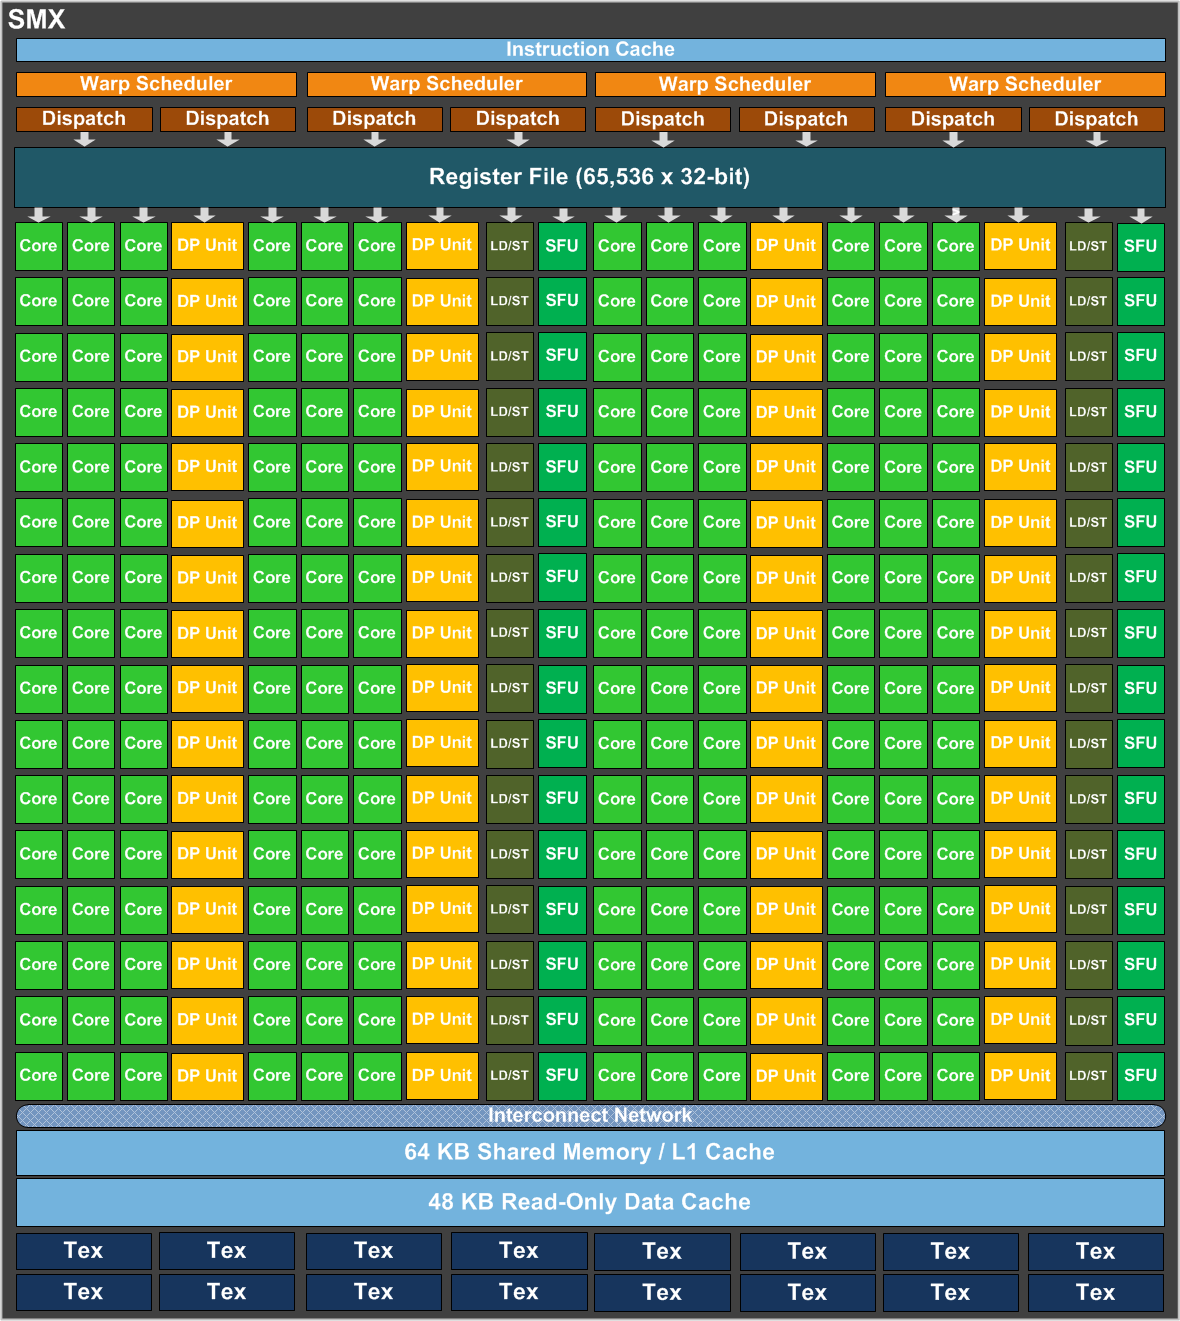
\includegraphics[width=0.9\textwidth]{kepler_arch_smx}
\caption{Architecture of a Streaming Multiprocessor (SMX) of NVIDIA's Kepler GK110 architecture containing 192 single precision CUDA cores, 64 double precision units, 32 special function units (SFU), and 32 load/store units (LD/ST) \cite{kepler_arch}.}
\label{fig:kepler_arch_smx}
\end{figure}

In figure \ref{fig:kepler_arch} we can see the design of a modern GPU by the example of NVIDIA's Kepler architecture. On the top side of the block diagram the PCI Express controller is placed. This interface is responsible for the communication of the graphics card with the CPU through the mainboard's PCI Express bus. After data has arrived at the graphics device, it has to be scheduled for processing to one or more of the streaming multiprocessors (SM, or SMX in NVIDIA's Kepler architecture terms). A SM is an aggregation of many cores with additional scheduling logic and therefore representing an extra hierarchical step in a GPU's workflow. This is one of the first bigger differences in the architecture of modern GPUs when compared with traditional CPUs. SMs are called compute units in OpenCL terms.

Figure \ref{fig:kepler_arch_smx} shows a detailed view of the structure of a streaming multiprocessors. Once a package of work is scheduled to a SM, it is then prepared for execution by the Warp Schedulers. A Warp is a block of threads (32 on NVIDIA hardware) executing the same instructions in parallel along cores managed by the Warp Scheduler. This concept is sometimes called SIMT (Single Instruction Multiple Threads). The difference to SIMD (Single Instruction Multiple Data) is that SIMD requires a vector instruction in each thread whereas SIMT only uses scalar code; the vectorization is handled by the hardware \cite[p.99]{gpu_optimizations}. A Warp Scheduler is able to manage multiple Warps at the same time (up to 64 on the Kepler GK110 architecture \cite[p.7]{kepler_arch}), which may be executed interleaved on the cores (similar to the two threads on a hyper-threading Intel core). This allows to hide memory latency (latency tolerance), because when a Warp has to stall because of a memory request, the Warp Scheduler can execute other Warps until the memory request is satisfied.

%\begin{figure}
%\centering
%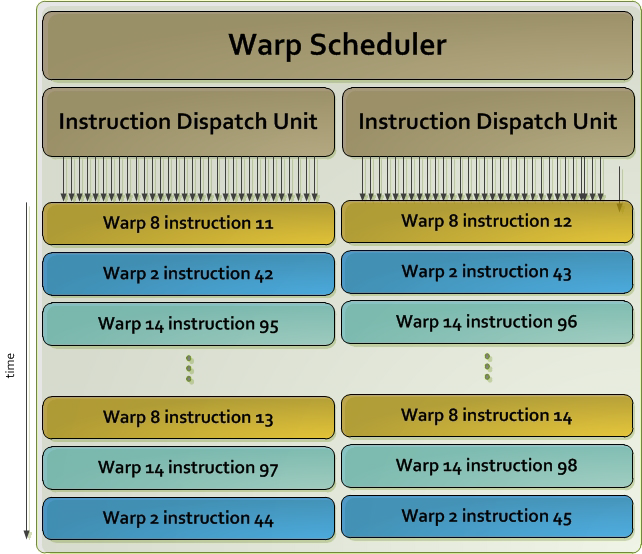
\includegraphics[width=0.5\linewidth]{warp_scheduler}
%\caption{Closer look on a Warp Scheduler. Each Warp Scheduler has two dispatcher units %allowing the execution of two independent instructions of a Warp in parallel. %\cite{kepler_arch}}
%\label{fig:warp_scheduler}
%\end{figure}

Another important thing to notice is that all cores within a SM share the same registers. This plays an important role when choosing the right number of Warps to run concurrently on the SM. Too less Warps may result in unused core cycles whereas a too large number of Warps may request more registers than there are available at the SM. The additionally needed registers are then allocated in the slow global memory. This concern will be discussed later in chapter \ref{sec:execution_model}.

The actual work is then performed on the cores itself. The major number of cores (labeled "Core" in green in figure \ref{fig:kepler_arch_smx}) are used for single precision floating point and integer arithmetics. In contrast to older GPUs, modern graphics processing units also include support for double precision floating point arithmetic, which was not needed for graphical calculations in the past, but becomes increasingly important in GPGPU computing. The Kepler architecture serves this need by dedicated cores (labeled "DP Unit"). Additional hardware resources include the load and store unit for register and memory access and the special function unit (labeled "SFU"). On the bottom of figure \ref{fig:kepler_arch_smx} we find the texture units which are heavily used in 3D graphics. They can also be used by OpenCL via images (more in chapter \ref{sec:images}).

Finally, beside the way of executing threads on its cores, the memory system is the second aspect of a GPU that shows significant differences to a CPU. Although also using a hierarchical cache system, the GPU lacks caches for each individual core. The first level cache resides within the SM and is used by all cores inside the SM. A specialty of the GPU is the shared memory (also scratch pad memory or local memory), which can be seen as a programmer controllable cache. An OpenCL kernel may use this small block of memory to cache data from the global memory and to limitedly share data with other threads (more on this in chapter \ref{sec:kernel_execcution}). Furthermore, shared memory is implemented in hardware using multiple memory banks. Special access patterns are required to avoid so-called bank conflicts resulting in slow memory request serialization between threads. Outside the SM (cf. figure \ref{fig:kepler_arch}) the GPU offers a larger level two cache which is then connected to multiple memory controllers to access the global memory. The global memory resides on the graphics card outside the GPU chip (such as the RAM is outside a CPU) and has a larger size of up to several GiB. An important difference of the global memory when compared with the RAM on the mainboard is that RAM can be accessed in almost any pattern without significant performance penalties (apart from cache effects). This is very different for a GPU where memory requests should be coalesced\footnote{A coalesced memory access occurs when all threads of a Warp request data on consecutive memory addresses resulting in a fast memory block transfer instead of individual transfers of smaller chunks. Most GPU hardware architectures have their global memory organized in segments of 64 or 128 bytes where always the full segment has to be transferred regardless of the size of the actually needed data \cite[p.13]{nvidia_opencl_best_practices}. Coalesced and aligned (guaranteed by compiler) memory access ensures to always transfer the minimum needed segments.} and blocked across the threads of a warp to achieve optimal memory system utilization.

Concerning the performance of a GPGPU accelerated application, there are a huge amount of concerns to worry about. Two of them have already been discussed, namely choosing the right number of warps concurrently executing on the SMs and paying attention to memory access. For the latter, the memory access pattern should be coalesced and frequently needed or shared data should be cached in shared memory. Further optimizations exist but would exceed the scope of this thesis. For further reading, NVIDIA has a detailed paper on this subject \cite{gpu_optimizations}.

AMD GPUs are structured similarly as the NVIDIA Kepler architecture presented here. A small difference is that AMDs Ultra-Threaded Dispatch Processor replaces the Warp Schedulers and schedules Wavefronts of 64 threads instead of 32 thread Warps. However, the most fundamental difference is found on instruction level. Whereas NVIDIA's cores only process one instruction at a time across a Warp, AMD processes a full packet of instructions in parallel. These packets are referenced to as VLIWs, or Very long instruction words. VLIWs are packets of four (or five on older GPUs) instructions that can be executed in parallel (instruction level parallelism). These packets are generated by the compiler. Due to dependencies between instructions, a VLIW may not always be completely filled and therefore not utilize a VLIW processor completely. Moving instruction level parallelization into the compiler is advantageous for the hardware, as it becomes simpler compared to hardware which tries to parallelize the instruction stream at run time via superscalar or out-of-order execution. Kepler's Warp schedulers for example can issue two instructions in parallel but have to resolve data dependencies between them at runtime via scoreboarding\footnote{Scoreboarding is a technique of processors where data dependencies of all instructions are tracked and instructions are only issued for execution if all dependencies have been resolved. Therefore, instructions may be reordered and executed in a different order.} \cite[p.4]{cayman_arch}. However, static scheduling might not be as efficient as scheduling at runtime as the compiler cannot make any assumptions about the occupancy of different pieces of hardware and thereof resulting delays. For further details about AMD's GPU architectures, David Kanter wrote a good article on real world technologies about AMD's Cayman architecture from 2010 with several comparisons to NVIDIA's Fermi architecture \cite{cayman_arch}.

\subsection{API Overview}

The OpenCL API is specified using the C programming language. The Khronos Group defines a set of C functions, types and constants that make up the API a developer can use to write applications using OpenCL. These declarations are cumulated into the cl.h C header file, which can be downloaded from the Khronos' website and can typically also be found in the include directory of any OpenCL SDK. Although specified in C, OpenCL has an object orientated design. The UML class diagram in figure \ref{fig:opencl_uml} shows the objects which can be created, queried and manipulated using corresponding API calls. The Khronos Group also specifies a C++ Wrapper with OpenCL 1.1 built atop the C API which will not be covered in this thesis.

The following chapters will give the reader a brief introduction into OpenCL's design and relevant API functions. The chapters are based on chapter 2 of the book Heterogeneous Programming with OpenCL \cite[p.15-31]{opencl_book}.

\begin{figure}
\centering
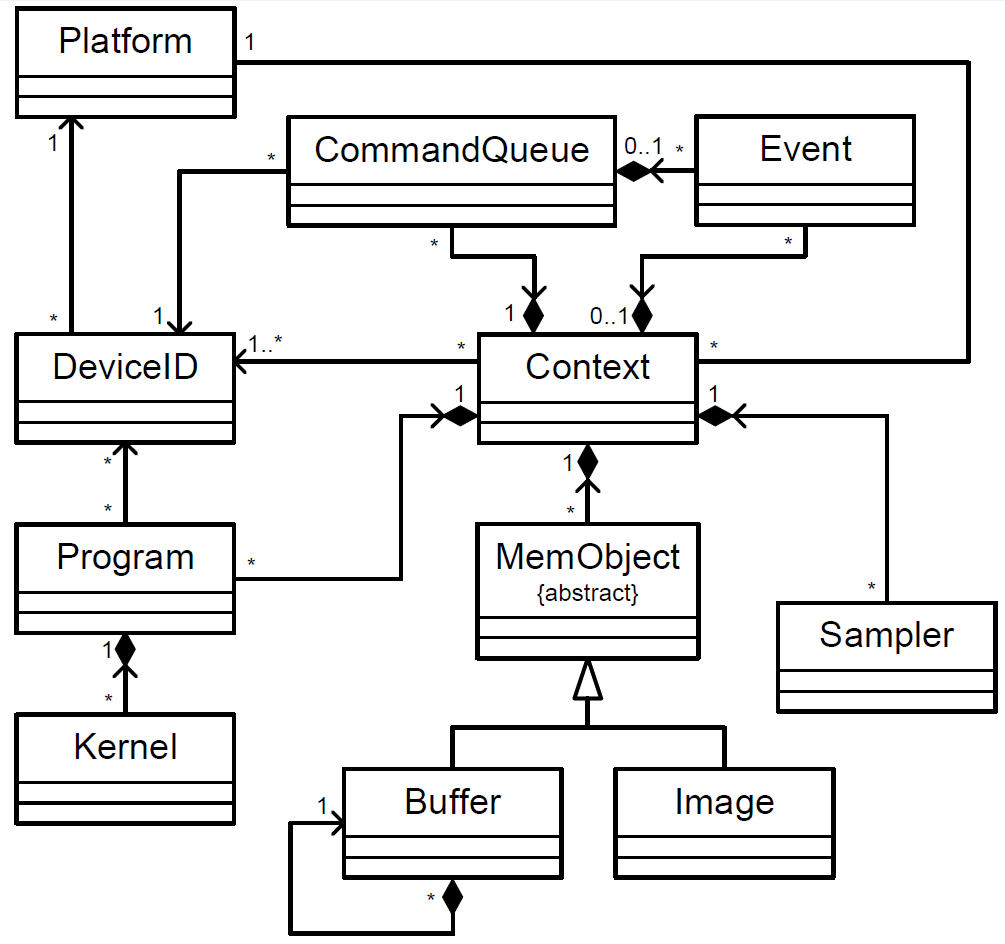
\includegraphics[width=0.6\textwidth]{opencl_uml}
\caption{OpenCL class diagram from the OpenCL 1.2 specification. \cite{opencl_spec}}
\label{fig:opencl_uml}
\end{figure}

\subsection{Platform model}
As OpenCL is an open standard it can be adopted by any hardware vendor manufacturing powerful enough processors to support the features specified by the Khronos Group. Many computers contain more than one of such processors; typically at least a CPU and a graphics card, which are both very suitable to be used by OpenCL. However, these devices do not have to share the same OpenCL implementation. On the one hand, someone may have an NVIDIA graphics card using NVIDIA's driver and, on the other hand, have an Intel Core using their OpenCL CPU driver. And then, if somebody has an AMD Radeon graphics card with AMD's Catalysts driver, the CPU can also be accessed using the same driver.
This situation of multiple available OpenCL implementations on the same machine is handled by the platform model. Each OpenCL implementation on the system (a vendor specific driver) represents a platform. The available platforms on the system, which in this context is often called the host, can be queried using the \lstinline!clGetPlatformIDs! function (for a source code sample see chapter \ref{sec:code_sample}).
Each platform supports one or more devices (the hardware supported by the driver). Reconsidering the previous scenario, the Intel platform would support one device, which is the CPU, whereas the AMD platform would support both the GPU and the CPU. The available devices of a platform can be retrieved by calling \lstinline!clGetDeviceIDs! with the desired platform. Devices available on the same platform (e.g. CPU and AMD GPU using the AMD platform) can be used together which is referred to as heterogeneous computing. 
A device itself consists of multiple compute units being functionally independent from each other (cf. the SMs of a GPU). Each compute unit itself is then eventually subdivided into processing elements (cf. the cores inside a SM). The number of available compute units on a device and much other information like memory capacities can be queried using \lstinline!clGetDeviceInfo!.
Figure \ref{fig:platform_model} visualizes the relation of platforms, devices, compute units and processing elements. \cite[p.19ff]{opencl_book}

\begin{figure} 
\centering
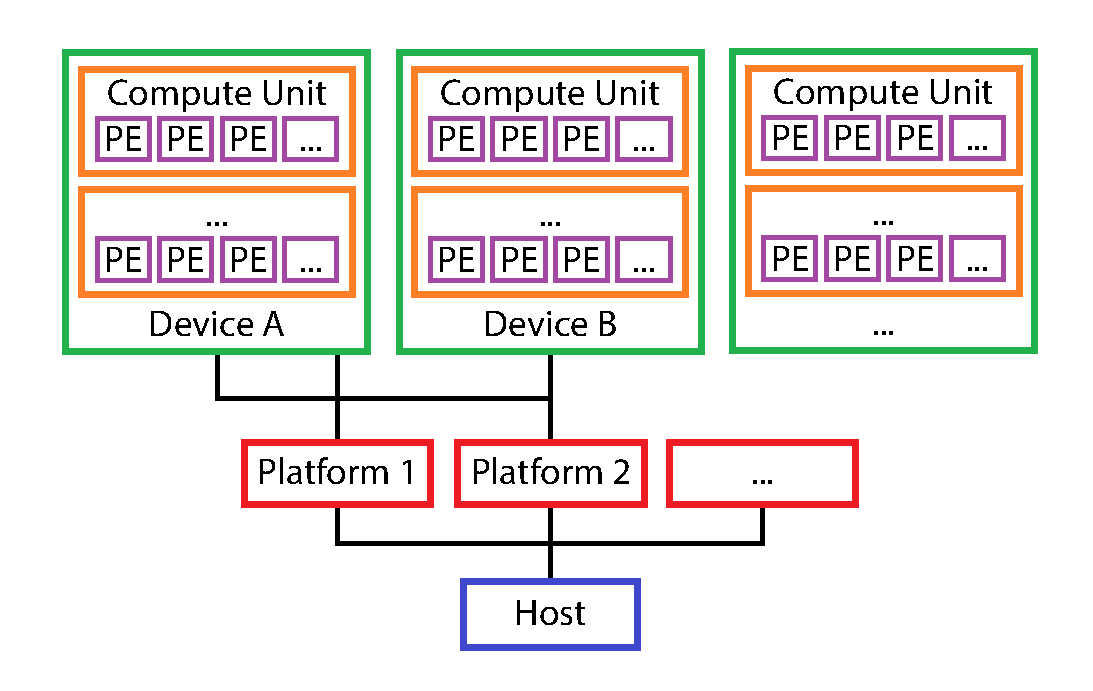
\includegraphics[width=0.7\textwidth]{platform_model}
\caption{OpenCL's platform model.}
\label{fig:platform_model}
\end{figure}

\subsection{Execution model}
\label{sec:execution_model}
The central component of OpenCL's execution model are kernels. But before a kernel can be executed on a device, a number of additional resources have to be set up.
After a device has been selected, a context has to be created that manages objects like memory buffers or kernels associated with the device. A context is created by calling \lstinline!clCreateContext! with one or more devices of the same platform as arguments. Additionally, properties may be passed to the function, like a platform to restrict the context to this platform allowing multiple contexts to different platforms to coexist, or a handle to an OpenGL (Open Graphics Library, a 3D API) context to enable graphics interoperability. \cite[p.22]{opencl_book}

While a context holds static objects shared between the host and one or more devices, OpenCL offers an additional mechanism for host device communication. To request action from a device, a command queue needs to be created within a context and associated with this device. This is done by calling \lstinline!clCreateCommandQueue! with the context and device as arguments. Once a command queue is created, the host can request actions from the device by enqueuing operations like memory buffer writes/reads or kernel executions. Per default these operations are executed asynchronously to the host application, although explicit synchronization can be enforced by calling \lstinline!clFinish! on the command queue, which blocks until all pending operations have been completed. \cite[p.22, 23, 26]{opencl_book}

\subsubsection{Creating kernels}
After the OpenCL execution environment has been successfully prepared, all that is left is the actual piece of code to execute. OpenCL C code is usually written into text files just as every other code. But in contrast to the host application, OpenCL C code is not compiled before an OpenCL application is deployed. OpenCL C code is compiled at runtime via corresponding API functions. This peculiarity is required as different vendors use individual binary codes that may be executed on their devices.
Therefore, an application has to read the OpenCL C code from the shipped source files at runtime and pass it to the \lstinline!clCreateProgramWithSource! function which returns a program object representing the given piece of code. This program can be compiled and linked for one or more devices by calling \lstinline!clBuildProgram!. As compile errors can occur (return value is not equal to \lstinline!CL_SUCCESS!) the compile log may be retrieved by a subsequent call to \lstinline!clGetProgramInfo!. After the program has been successfully built, kernels can be extracted (a program may contain multiple kernels). This is done by calling \lstinline!clCreateKernel! with the compiled program and the name of a function with the \lstinline!__kernel! attribute, which will be used as entry point into the kernel. The obtained kernel is ready for being enqueued on a command queue to a device the kernel was compiled for. \cite[p.26, 27]{opencl_book}

\subsubsection{Kernel execution}
\label{sec:kernel_execcution}
A kernel can be seen as C function that is executed in parallel on the device's processing resources by the OpenCL runtime. As elaborated in chapter \ref{sec:hardware_arch}, these resources may be organized very differently. Therefore OpenCL uses an abstraction model describing the dimensions of the queued work and how it is split up into small pieces. \cite[p.16]{opencl_book}

When the host application wants to enqueue a kernel, it has to specify the size of the problem as a so-called n-dimensional range (NDRange). This range can be seen as a one-, two- or three-dimensional grid of indexes which typically represent the size of the input or output of a kernel. Each element of the grid represents a single kernel invocation and is called a work item. Work items are identified by their position inside the grid which is named global id. The size of the grid is called the global work size. \cite[p.18]{opencl_book}

For example: a matrix multiplication with an output matrix of $M*N$ elements might enqueue a kernel with a two-dimensional range of $M*N$ work items. Each work item would then use it's indexes to determine the row and column of the input matrices and the position of the calculated output value.

To closer adapt to GPU hardware architectures, the NDRange can be equally divided into work groups. Work items inside a work group benefit from having a dedicated shared memory block available. Access to this memory can be synchronized between the work items of a work group providing a basic method of communication. To address a work item inside a work group, each work item has an additional local id and a group id. The extends of a work group must be of the same dimension as the NDRange and the sizes in each dimension, called local work sizes, must be powers of two and evenly divide the global work sizes. \cite[p.18]{opencl_book} The maximum number of work items in a work group is implementation dependent and can be queried by a call to \lstinline!clGetDeviceInfo! with the \lstinline!CL_DEVICE_MAX_WORK_GROUP_SIZE! constant as argument. Figure \ref{fig:NDRange} shows the relation of the NDRange, work groups and work items. 

\begin{figure} 
\centering
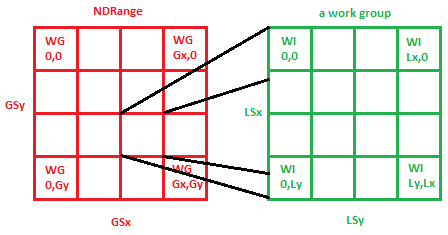
\includegraphics[width=0.6\linewidth]{NDRange}
\caption{The two-dimensional NDRange consisting of $GSx * GSy$ work groups. Each work group consists of $LSx * LSy$ work items. A work item has two indexes in each dimension, the local index (relative to the work group) and a global index (relative to the NDRange), as well as the indexes of the group it is part of. The local work sizes are LSx and LSy whereas the global work sizes are $GSx * LSx$ and $GSy * LSy$.}
\label{fig:NDRange}
\end{figure}

A kernel is executed on a command queue by calling \lstinline!clEnqueueNDRangeKernel!. Additional important arguments beside the kernel and the command queue are the NDRange's dimensions, the global work size and the local work size. The local work size is optional. Before a kernel is executed, arguments may be specified for the \lstinline!__kernel! function according to the function's signature. These arguments are passed to the device when the kernel starts executing and can be accessed via the \lstinline!__kernel! function's parameters. Arguments are set from the host by calling \lstinline!clSetKernelArg! with the argument's index in the kernel function's signature as well as the size and value of the argument.

\subsubsection{Kernel code}
The language kernels are written in is OpenCL C, which is derived from C99 and extended by OpenCL specifics like vector data types, built in functions and additional key words. A kernel function must have the \lstinline!__kernel! attribute and must have void as it's return type. The function's name identifies the kernel to the host. A kernel may have parameters which are declared in the function's signature. An example kernel function for a matrix multiplication is given in listing \ref{lst:kernel_example}.

\lstset{basicstyle=\ttfamily{}\scriptsize{}}
\begin{lstlisting}[caption={An example of a \lstinline!__kernel! function's signature.},label={lst:kernel_example}]
__kernel void matrixMultiplication(int n, int m, __global const float* matrixA, __global const float* matrixB, __global float* output) {
// kernel code ...
}
\end{lstlisting}
\lstset{basicstyle=\ttfamily{}}

\subsection{Memory}
Many applications often have to work with large amounts of data. As the data that can be passed to a kernel function by value is restricted to a small size, OpenCL offers the possibility to allocate larger blocks of memory represented as a memory object which is valid inside a context and moved to a device when necessary. At the very top OpenCL defines two basic types of memory, buffers and images. Buffers can be seen as a continuous block of memory equivalent to an array in C allocated using \lstinline!malloc!. Images in contrast are abstract memory objects which can make use of device specific hardware acceleration and optimization when being read from or written to (e.g. texture units on a GPU). Images do not have to be supported by a device. \cite[p.23f]{opencl_book}

\subsubsection{Buffers}
Buffers are created by the host application via a call to \lstinline!clCreateBuffer!. In addition to the context and buffer size, several flags may be specified. With these flags (beside further options) the buffer can be declared as read or write only, or OpenCL can be instructed to use or copy a provided block of host memory. Once a buffer is created, read and write operations may be enqueued on a command queue to transfer a buffer's content (or parts of it) between the host and a device. \lstinline!clEnqueueReadBuffer! and \lstinline!clEnqueueReadBuffer! are the corresponding API functions for transferring memory. When needed by a kernel, buffers have to be set as arguments to a kernel and can be accessed via a pointer from inside the kernel function. \cite[p.24]{opencl_book}

\subsubsection{Images}
\label{sec:images}
Images abstract the underlying storage implementation to allow a device to use hardware optimizations. GPUs for example might use their texture units for improved read and write access as well as providing hardware accelerated interpolation between pixel values of the image. As images do not need to be represented as continuous arrays of a specified data type, a format descriptor is used to determine the size and data type of a pixel value of the image. Images are created by a call to \lstinline!clCreateImage2D! or \lstinline!clCreateImage3D! (unified to \lstinline!clCreateImage! in OpenCL 1.2) with similar parameters as the buffer creating functions. Additionally, the image format descriptor has to be specified and an optional padding between the rows of the image can be set. Images are read and written by the host application via calls to \lstinline!clEnqueueReadImage! and \lstinline!clEnqueueWriteImage!. Like buffers, images can be set as arguments to a kernel, but cannot be accessed via pointers inside the kernel function. Special built-in functions like \lstinline!read_imagef! have to be used in combination with a sampler object which determines out-of-bounds image access, interpolation, and access coordinate handling. \cite[p.25f]{opencl_book}

\subsubsection{Memory model}
As memory subsystems are highly diverse between different kinds of hardware devices, OpenCL defines an abstract memory model giving vendors the possibility to map OpenCL's abstract types of memory to physical memory units on a device.
OpenCL defines four different types of memory which are shown in figure \ref{fig:memory_model}:

\begin{figure} 
\centering
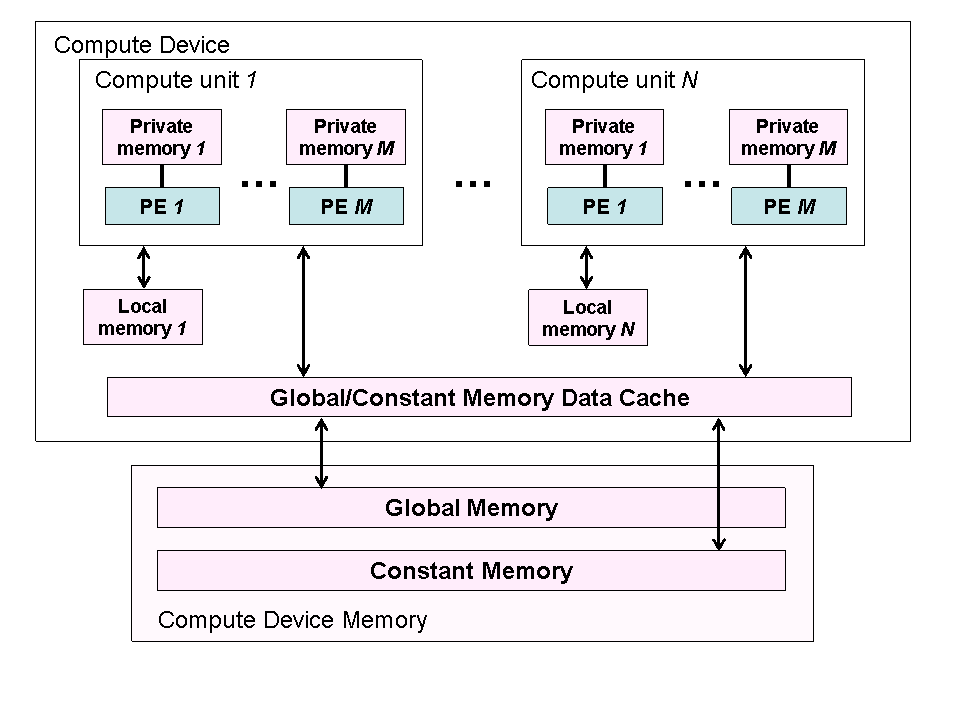
\includegraphics[width=0.6\linewidth]{memory_model}
\caption{Memory model as defined by the OpenCL 1.2 specification.\cite{opencl_spec}}
\label{fig:memory_model}
\end{figure}

\begin{description}
	\item[Global memory] \hfill \\
	Global memory is the largest of all memory regions and visible to all compute units on a device. This memory region is used whenever data is copied to or from a device. Buffers and images are allocated in this memory. All pointer variables pointing into global memory have to be prefixed with the \lstinline!__global! attribute inside a kernel. \cite[p.29]{opencl_book}
	
	\item[Constant memory] \hfill \\
	Constant memory is typically implemented as part of the global memory and is used to store read only data which is needed by all work items. All pointer variables pointing into constant memory have to be prefixed with the \lstinline!__constant! attribute inside a kernel. \cite[p.30]{opencl_book} Newer types of hardware may provide special caches for this kind of memory (cf. the read-only data cache in NVIDIA's Kepler architecture in figure \ref{fig:kepler_arch}).
	
	\item[Local memory] \hfill \\
	Local memory (or shared memory) is a small block of memory which is shared between all work items inside a work group. As access to local memory is very fast it can be seen as a programmer controlled cache to global memory. Local memory is often used for preloading data needed by all work items of a work group or to synchronize work items across a work group. All pointer variables pointing into local memory have to be prefixed with the \lstinline!__local! attribute inside a kernel. Local memory can be allocated statically inside a kernel by declaring a fixed sized array like \lstinline!__local float sharedArray[32];! or dynamically with a call to \lstinline!clSetKernelArg! providing the size of the local memory block requested and \lstinline!nullptr! as pointer to the arguments value. \cite[p.30]{opencl_book}

	\item[Private memory] \hfill \\
	Private memory belongs to each work item itself and is typically stored in registers (on a GPU) except a work group requests more memory than the available register file. In this case the spilled private memory is mapped to global memory. Private memory cannot be allocated, but pointers to local variables may be used to pass values by reference to functions called by the kernel function. Pointers to variables pointing to private memory can be prefixed with the \lstinline!__private! attribute inside kernels, but they do not have to as \lstinline!__private! is the default pointer type. \cite[p.30]{opencl_book}
\end{description}

\subsection{Code sample}
\label{sec:code_sample}

The following piece of code in listing \ref{lst:opencl_example} shows a minimal OpenCL application with a kernel that calculates the sum of two input vectors. To keep the code simple no error handling is performed, only the error code is retrieved. The codes in the subsequent implementation chapters will completely go without error handling or error code retrieval.

\pagebreak

\lstset{basicstyle=\ttfamily{}\scriptsize{}}
\lstinputlisting[language=C++,caption=A minimalistic working OpenCL application which calculates the sum vector of two large input vectors.,label=lst:opencl_example]{code/sample/main.cpp}
\lstset{basicstyle=\ttfamily{}}

The first step in every OpenCL program is to choose a platform. As platforms correspond to the available OpenCL implementations on the system, multiple platforms can be available. The example code only queries the first available OpenCL platform by calling \lstinline!clGetPlatformIDs! with 1 and a pointer to a variable able to hold one platform id as arguments. The third parameter could be used to retrieve the number of actually available platforms. \\
After a platform has been chosen, we can continue by choosing a device for this platform which works analogously as selecting a platform. In addition to specifying the platform to query devices for, OpenCL also allows us to define the type(s) of devices we would like to get. In this case we would like to have the first available GPU on the first available platform by specifying \lstinline!CL_DEVICE_TYPE_GPU! when calling \lstinline!clGetDeviceIDs!\footnote{Calling \lstinline!clGetDeviceIDs! with a device type as argument may return no devices. The Intel OpenCL platform for example only supports CPUs and therefore does not provide a GPU device. Appropriate error handling is necessary in real world applications.}. To be able to allocate OpenCL resources and enqueue operations on a device we now have to create a context and a command queue using \lstinline!clCreateContext! and \lstinline!clCreateCommandQueue!. Further arguments to both API functions allow specifying further properties which can be looked up in the corresponding documentation. \\
The program is now ready to create a kernel. OpenCL kernel source code is typically placed in a file and read at runtime. For simplicity, the kernel code of this example is emplaced into the host code as string literal. The OpenCL kernel simply queries the id of the current work item, loads the values from the buffers \lstinline!a! and \lstinline!b! at this index and writes the sum of them to buffer \lstinline!c! at the same index. \\
To create an actual kernel object within the context, we first have to create an OpenCL program out of the source code which is done by calling \lstinline!clCreateProgramWithSource! and passing the source code as argument. Furthermore, the program has to be compiled for the chosen device. By calling \lstinline!clBuildProgram! the source code of the program object is compiled and linked into an executable for the specified device. This step can take up to several seconds. Similar as building programs in other languages, the compiling may fail. In this case an error code is returned and a compiler log could be retrieved using \lstinline!clGetProgramBuildInfo!.
On a successful build, the kernel object (which can be seen as entry point into the program) can be finally retrieved by calling \lstinline!clCreateKernel! and specifying the compiled program as well as the name of the \lstinline!__kernel! function. \\
Before we can execute the kernel we have to allocate storage for the input and output data. Three arrays are allocated on the host with a size of \lstinline!N!. The first two are filled with data. To move the data to the GPU, three buffer objects have to be created using \lstinline!clCreateBuffer! having the same size as the corresponding host arrays. Note that the two input buffers are created as read only and the output buffer as write only by setting appropriate flags. To initiate the copy operations from the host to the GPU device, buffer write operations have to be enqueued on the command queue using \lstinline!clEnqueueWriteBuffer!. Arguments are the command queue, the buffer to write to, a boolean specifying if the write operation should be blocking, the offset and length of the region to be written to, a pointer to the host memory from which should be read and several further arguments concerning events which will not be covered. By specifying \lstinline!false! for the blocking write parameter, the write operation is execute asynchronously to the host program. Therefore the provided host pointers (\lstinline!a! and \lstinline!b!) have to be available at least until the first blocking OpenCL call. Asynchronous memory transfers are advantages, as OpenCL may decide itself when to perform the actual copy. Furthermore, multiple copies may be executed concurrently and even beside kernel executions.\\
Now it is time to setup and execute the kernel. The three buffer objects, on which the kernel will operate, are set as the kernel's arguments via \lstinline!clSetKernelArg!. The second parameter specifies the index of the argument in the order they appear in the kernel function's signature. Finally, the kernel can be enqueued to be executed using \lstinline!clEnqueueuNDRangeKernel!. The problem is one-dimensional with a global work size of \lstinline!N!. The local work size is not specified and therefore determined by OpenCL. Similar to the buffer writes, the kernel enqueue operation is also executed asynchronously. However, the arguments do not have to be available anymore after \lstinline!clSetKernelArg! returns as they are copied by the OpenCL implementation. Furthermore, as the kernel depends on the buffer objects as inputs, the kernel is not executed until all buffer operations (memory transfers) on the inputs have completed. \\
The last step is to read the results back to host memory via \lstinline!clEnqueueReadBuffer! having the same arguments as the corresponding write function. This time however, the synchronization boolean is set to \lstinline!true!. Therefore, the function call blocks until the read operation has finished. Afterwards the result on the host may be further processed (e.g. printed). \\
When OpenCL resources are no longer needed, they should be released using their corresponding \lstinline!clRelease*! API functions.

\section{Matrix multiplication}

Multiplying matrices of a large size is often part of heavy scientific calculations and therefore an important building block in every mathematics library. Unfortunately, with an increasing size of the matrices the computation of the product becomes desperately slow due to an asymptotic runtime complexity of $\mathcal{O}(n^3)$ for a naive attempt. Therefore, several improvements have been tried to speed up the calculation like Strassen's algorithm achieving a runtime complexity of $\mathcal{O}(n^{\log_2 7}) = \mathcal{O}(n^{2.807})$ \ref{} which is faster than the naive version but still does not compute results within a satisfying time.
Nonetheless, modern computing systems can take advantage of one important aspect of the matrix multiplication which is it's embarrassing parallel nature. Each element of the output matrix can be computed completely independent. This potential may not only be used by today's CPU's vector extensions like SSE \footnote{Streaming SIMD Extensions, a vector instruction set extension by Intel supporting 128 bit wide registers to process 4 single precision floats in parallel.} or AVX \footnote{Advanced Vector Extensions, Intel's latest vector instruction set extension featuring 256 bit wide registers to process 8 single precision floats in parallel.}. Especially a GPU can make excellent use of the large number of independent pieces of work to perfectly utilize its hundreds or thousands of cores.

\begin{figure}
\centering
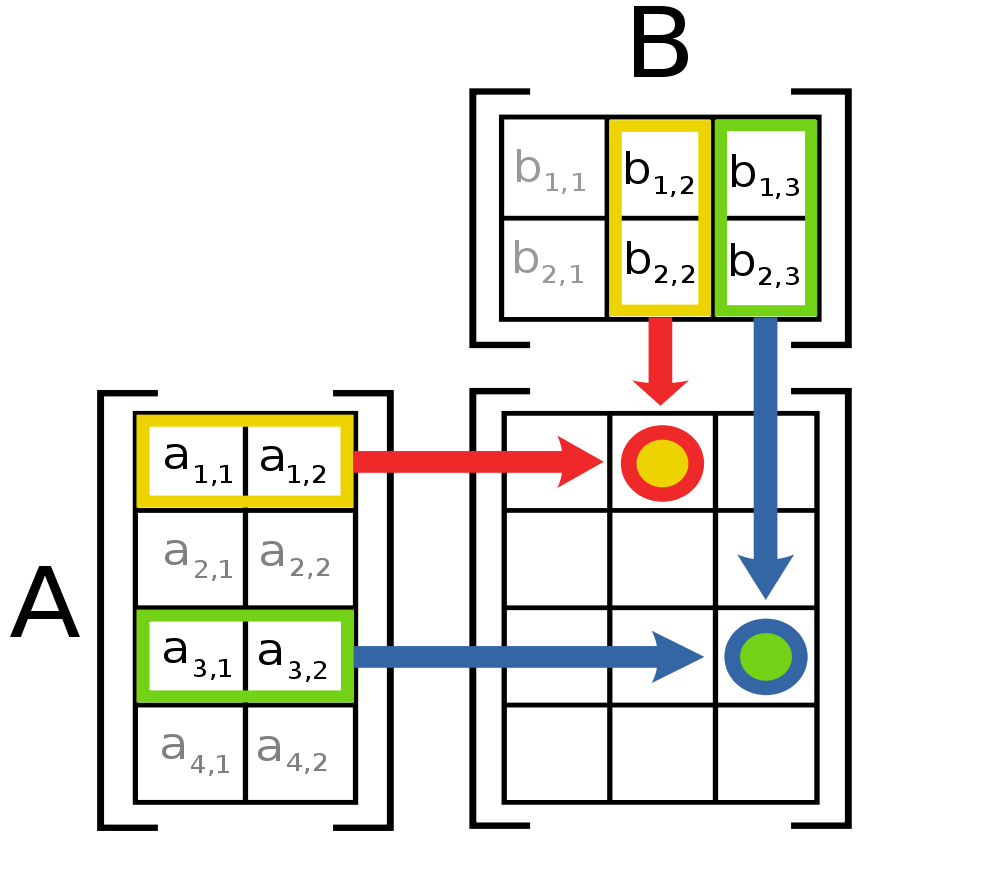
\includegraphics[width=0.5\linewidth]{matrix_mul}
\caption{Principle of the matrix multiplication \cite{wiki_matrix_mul}.}
\label{fig:matrix_mul}
\end{figure}

This chapter will take a look at different implementations of the matrix multiplication for both, the CPU and the GPU. For simplicity, square matrices are used and stored as one dimensional arrays in row major order.

\subsection{CPU Implementation}
\label{sec:matrix_cpu_implementation}

Although several optimized implementations exist we will first have a detailed look at a simple naive implementation as given in listing \ref{lst:matrix_cpu}.

\lstset{basicstyle=\ttfamily{}\scriptsize{}}
\lstinputlisting[language=C++, caption=A simple C++ implementation of a square matrix multiplication for the CPU., label=lst:matrix_cpu, firstline=15, lastline=26]{code/matrix/main.cpp}
\lstset{basicstyle=\ttfamily{}}

The \lstinline!matrixMul()! function takes two pointers to the memory where the two input matrices are stored, another pointer to already allocated memory where the output is written to and a final \lstinline!size! parameter giving the edge length of the input and output matrices.
The algorithm itself is simple. Every element of the output matrix has to be calculated, therefore the outer two \lstinline!for! loops run through all of these elements. For each output element the dot product of the \lstinline!row! in matrix \lstinline!a! and the \lstinline!col! in matrix \lstinline!b! are calculated.

The performance of this implementation is conceivably slow as one can see in figure \ref{fig:matrix_chart}. Multiplying matrices with an edge length of up to 700 elements can be done in a short time (below one second), but larger matrices require a huge period of time which is unsatisfying in most cases.

\subsection{Naive GPU implementation}

A working GPU implementation can be directly derived from the simple CPU implementation given in the previous chapter \ref{sec:matrix_cpu_implementation}. As we can see in figure \ref{fig:matrix_mul}, each output element is calculated independently and the calculation of an output element corresponds to the loop body of the second \lstinline!for! loop in the CPU implementation in listing \ref{lst:matrix_cpu}. Therefore, both outer \lstinline!for! loops offering a good starting point for parallelization. 

The naive GPU implementation seen in listing \ref{lst:matrix_cl_naive} uses the same principle as the initial CPU version. To simplify the code listing context and command queue have already been created and are provided as input to the \lstinline!matrixMulCL()! function.
For the three buffers holding the two input matrices and the output matrix OpenCL buffers have to be created. On creation, additional flags may be provided to allow the underlying OpenCL implementation to optimize memory access to these buffers. Therefore, the two input matrix buffers are set to \lstinline!CL_MEM_READ_ONLY! and the output buffer is set to \lstinline!CL_MEM_WRITE_ONLY!. These flags only affect access to the memory object from the kernel code and do not restrict the host application to read or write buffers. 
After the buffers have been created, a write operation is enqueued on the command queue to the GPU for both input matrices. Note, that the third parameter of the calls to \lstinline!clEnqueueWriteBuffer()! specifies whether the function blocks until the write operation has completed or not. This parameter is set to \lstinline!false! allowing OpenCL to transfer the memory blocks asynchronously to the running host application and even in parallel .
Before the kernel can be executed, the two input buffers, the output buffer and the size of the matrix are set as arguments to the \lstinline!__kernel! function. Furthermore the global and local work size for the kernel execution have to be determined. The global work size must be a multiple of the used work group size (local work size). The chosen size of the work groups affects GPU utilization as a too small size may lead to wasted processing powers on the SMs and decreases latency tolerance. A too large work group size may cause the kernel to fill up the available register file on the SM in which case local variables are moved to global memory causing a serious drop in performance. Finding the optimal work group size is strongly hardware dependent and often boils down to simple try and error.
Note that choosing a work group size which does not evenly divide the global work size and therefor rounding the global work size to the next multiple of the work group size causes the GPU to execute the kernel for additional unneeded work items. Concerning the matrix multiplication example, the kernel would be executed for a bigger matrix with an edge length evenly dividable by the work group size. This has to be kept in mind when e.g. accessing buffers inside the kernel.

After global and local work size have been chosen, the kernel can be enqueued on the command queue to be executed by calling \lstinline!clEnqueueNDRangeKernel()!. The call immediately returns as the kernel is executed asynchronously when the command queue is flushed (\lstinline!clFlush()!) or a blocking command is enqueued, which is the case on the subsequent read operation. The call to \lstinline!clEnqueueReadBuffer()! reads the result back from the device to the host application's array. Note that the third parameter is set to \lstinline!true! indicating a blocking operation. All previously enqueued commands are ensured to be executed and finished before the read operation takes place which returns after all data has been successfully copied to client memory.

\lstset{basicstyle=\ttfamily{}\scriptsize{}}
\lstinputlisting[language=C++, caption=Host code for a matrix multiplication implementation using OpenCL., label=lst:matrix_cl_naive, firstline=29, lastline=55]{code/matrix/main.cpp}
\lstset{basicstyle=\ttfamily{}}

The last missing component of the naive GPU implementation is the OpenCL kernel itself which is given in listing \ref{lst:matrix_cl_naive_kernel}. The \lstinline!__kernel! function closely resembles the loop body of the second \lstinline!for! loop of the CPU implementation in listing \ref{lst:matrix_cpu}. The purpose of a single invocation of this kernel is to calculate one element of the output matrix. By using OpenCL's built-in function \lstinline!get_global_id()! with the dimension as argument, the kernel invocation can retrieve it's position inside the NDRange which equals the output matrix (plus extra space due to work group size rounding). Therefore, the retrieved position has to be checked against the matrices' size as the NDRange may be larger than the original matrix. If the coordinates identify a valid matrix position, the output element is again determined by calculating the dot product of the \lstinline!row! in matrix \lstinline!a! and the \lstinline!col! in matrix \lstinline!b! and eventually written to the output matrix buffer \lstinline!c!.

\lstset{basicstyle=\ttfamily{}\scriptsize{}}
\lstinputlisting[language=CL, caption=OpenCL Kernel code calculating a single element of the output matrix., label=lst:matrix_cl_naive_kernel]{code/matrix/Mult.cl}
\lstset{basicstyle=\ttfamily{}}

When run on the GPU, the performance of this naive OpenCL implementation is already amazingly fast when we have a look at the benchmark in figure \ref{fig:matrix_chart}. At an edge length of 800 elements, the size where the CPU implementation's needed time started to blow up beyond several seconds, the GPU variant still runs very happily at around 200 milliseconds. Additionally, the curve raises far slower than the CPU's one.


\subsection{Optimized GPU implementation}
options for performance improvement
multiple elements per work item

texture unit

\subsubsection{Using vector instructions}
vector instructions (AMD Tile)


\subsubsection{Using local memory}
caching in local memory (blocks)

\subsection{Existing implementations}

Beside the presented implementations, several libraries exist supporting matrix multiplication.

\begin{description}
   \item[clAmdBlas] \hfill \\
   A BLAS (Basic Linear Algebra Subprograms) library provided by AMD.
   \item[cuBlas] \hfill \\
   A BLAS (Basic Linear Algebra Subprograms) library provided by NVIDIA shipped with the CUDA Computing SDK.
\end{description}

\subsection{Benchmarks and conclusion}
Which implementation is when better?

\begin{figure}
\centering
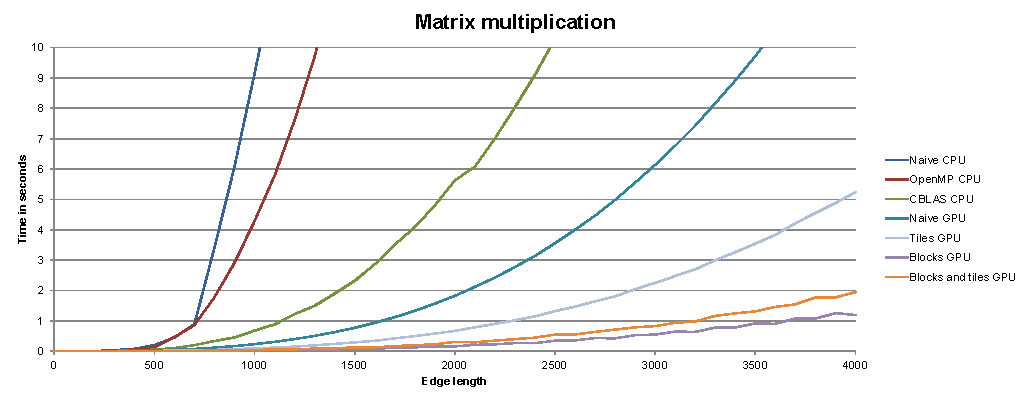
\includegraphics[width=1.0\linewidth]{matrix_chart}
\caption{Benchmark of several square matrix multiplication implementations. CPU implementations are drawn as dashed lines.}
\label{fig:matrix_chart}
\end{figure}

Which problem size?
Which hardware?



\chapter{Prefix sum}
\label{sec:prefix_sum}

The all-prefix-sums operation (also referred to as prefix sum or simply scan) is a simple calculation which is most often found as part of larger and more complex routines. It serves as fundamental building block for implementing well-known algorithms such as radix sort (covered in section \ref{sec:sorting_radix}), stream compacting, minimum spanning tree and many more (cf. Blelloch's papers on prefix sum \cite{scan_blelloch_examples} \cite{scan_blelloch} and the GPU Gems 3 book section 39.1 \cite{gpu_gems_3_chapter_39}).

The all-prefix-sums operation uses a binary, associative operator $\oplus$ with identity element $I$ to transform an input array of $n$ elements
\begin{equation*}
[a_0, a_1, \dots, a_{n-1}]
\end{equation*}
into an output array of $n$ elements where

\begin{enumerate}[label=\alph*)]
	\item 
	each output element is the sum of all elements preceding the corresponding input element. This is known as an exclusive scan. \cite{gpu_gems_3_chapter_39}
	\begin{equation*}
	[I, a_0, (a_0 \oplus a_1), \dots, (a_0 \oplus a_1 \oplus \dots \oplus a_{n-2})]
	\end{equation*}
	
	\item
	each  output element is the sum of all elements preceding the corresponding input element and the input element itself. This is known as an inclusive scan. \cite{gpu_gems_3_chapter_39}
	\begin{equation*}
	[a_0, (a_0 \oplus a_1), \dots, (a_0 \oplus a_1 \oplus \dots \oplus a_{n-1})]
	\end{equation*}
\end{enumerate}

Contrary to the matrix multiplication of chapter \ref{sec:matrix_mul}, the all-prefix-sums operation does not offer similarly trivial parallelism. Scanning an array is naturally sequential with a complexity of $\mathcal{O}(n)$. Although each output element could be calculated independently to gain parallelism, a lot of redundant work would be necessary raising the overall complexity to $\mathcal{O}(n^2)$ with the last element still taking $\mathcal{O}(n)$ time to calculate.
This chapter will focus on efficient and parallel implementations of exclusive scan (except otherwise noted) using addition as operator on an input array of signed 32 bit integers. This chapter is orientated towards the Parallel Prefix Sum article from GPU Gems 3 \cite{gpu_gems_3_chapter_39}.


\section{CPU Implementation}
\label{sec:scan_cpu}

Implementing a sequential, single threaded scan for the CPU is simple. The first output element is initialized to zero. We than loop over the remaining output elements and set each one to the value of its predecessor plus the corresponding input element. Listing \ref{lst:scan_cpu} presents an example of a scan implementation.

\lstset{basicstyle=\ttfamily{}\scriptsize{}}
\lstinputlisting[language=CPP, caption=A simple C++ implementation of an exclusive scan for the CPU., label=lst:scan_cpu, firstline=34, lastline=38]{code/scan/main.cpp}
\lstset{basicstyle=\ttfamily{}}

This code performs exactly $n - 1$ additions which is the minimum number of additions required to produce an exclusive scan of an array with $n$ elements. Concerning the following parallel scan implementations later in this chapter, we would like them to be work-efficient. This means that the parallel implementation should have the same work complexity of $\mathcal{O}(n)$ as the sequential one.

\begin{quote}
A parallel computation is work-efficient if it does asymptotically no more work (add operations, in this case) than the sequential version \cite{gpu_gems_3_chapter_39}.
\end{quote}

The benchmark of this algorithm in figure \ref{fig:scan_chart} confirms the linearity of scan. Furthermore, we can also see that scanning is a quite fast operation (when, e.g., being compared to the matrix multiplication of chapter \ref{sec:matrix_mul}). The CPU implementation manages to scan $2^{26}$ elements (256 MiB of data) in 225 ms.

\begin{figure}[!p]
\centering
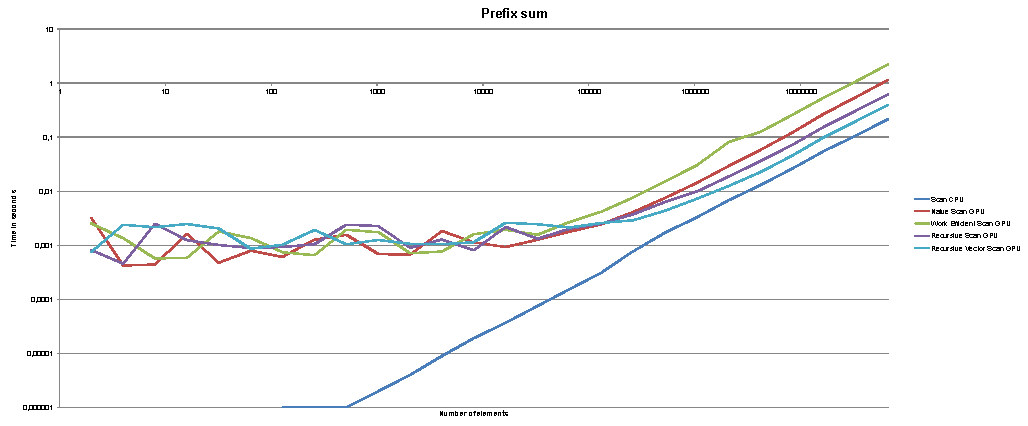
\includegraphics[width=0.9\textheight, angle=90]{scan_chart}
\caption{Benchmark of several prefix sum implementations, where
%The chart is based on the benchmark data in appendix section \ref{sec:scan_chart_data}.
both axes are of logarithmic scale.}
\label{fig:scan_chart}
\end{figure}

\section{Naive GPU implementation}
\label{sec:scan_naive}

The first GPU implementation is base on the article Data Parallel Algorithms \cite{scan_naive}. The discussed approach is to compute an inclusive (!) scan is shown in figure \ref{fig:scan_naive}. The algorithm uses several passes to compute the final output array in place. In each pass the value of a predecessor is added to an element. The offset from each element to its predecessor is determined by the pass index and is $2^{d - 1}$ where d is the number of the pass starting with 1.

\begin{figure}[h]
\centering
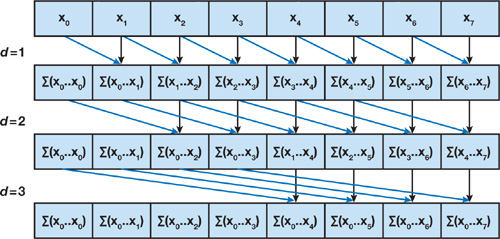
\includegraphics[width=0.6\textwidth]{scan_naive}
\caption{A naive approach for a parallel scan. \cite{gpu_gems_3_chapter_39}}
\label{fig:scan_naive}
\end{figure}

By now the algorithm assumes that in each pass all input elements are read before any output elements are written. This can only be achieved if this algorithm is run on a device with as many cores as input elements to ensure correct read and write ordering. This is usually not the case for larger arrays (current GPUs have around a few thousands cores. cf. NVIDIA Kepler GK110 in section \ref{sec:gpu}). A solution to this problem is double buffering. Instead of computing the partial sums in place inside the input array, a second, equally sized buffer is created. In each pass input data is read from one of the buffers and written to the other. Before the next pass the buffers are swapped.
Listing \ref{lst:scan_naive_host} shows an example host code implementing this approach.

\lstset{basicstyle=\ttfamily{}\scriptsize{}}
\lstinputlisting[language=CPP, caption=Host code for the naive scan algorithm., label=lst:scan_naive_host, firstline=40, lastline=64]{code/scan/main.cpp}
\lstset{basicstyle=\ttfamily{}}

At first, two buffers with the size of the input are created. Both of them have to be read- and writable as they are read from and written to alternatingly when executing the passes. The source buffer is filled with the input data. Although this algorithm is independent from the chosen work group size, we have to round the number of enqueued work items (one for each input element) up to be a multiple of the work group size, which will be the size of the enqueued ND range. After this short setup the passes are executed. Each pass corresponds to a power of two (loop variable \lstinline!offset!, cf. figure \ref{fig:scan_naive}) which corresponds to the offset of an element to the predecessor that should be added to it. This offset is raised to the next power of two each pass until it is larger than the problem size. The kernel is executed once for each pass, given the source and destination buffer, the offset and the original problem size as arguments. At the end of a pass the source and destination buffers are swapped (only the handles, not the actual contents). After the last pass has been executed, the result is read from the source buffer (the last pass wrote to the destination buffer which was swapped with the source buffer at the end of the loop).
Listing \ref{lst:scan_naive_kernel} shows the kernel code corresponding to the host code from listing \ref{lst:scan_naive_host}.

\lstset{basicstyle=\ttfamily{}\scriptsize{}}
\lstinputlisting[language=CL, caption=OpenCL Kernel code for the naive scan algorithm., label=lst:scan_naive_kernel]{../src/scan/gpu/thesis/NaiveScan.cl}
\lstset{basicstyle=\ttfamily{}}

\pagebreak

The kernel starts by querying the id of the current element. If this id is larger than the actual problem size, the kernel returns. This case can happen when the problem size has been rounded up to be a multiple of the chosen work group size. If the id addresses a valid input element, we determine if this element has a predecessor at the current pass' offset. If this is the case, the input element is read from the source buffer, added to its predecessor (also read from the source buffer) and written to the destination buffer. If the predecessor offset is to large, the input element remains the same, but has to be copied if it was just calculated in the last pass (to keep the buffers consistent).

When we have a look at the benchmark of this algorithm and compare the results with the CPU implementation, we can clearly see that this approach does not profit very well from the large computational power GPUs offer. With 1132 ms at $2^{26}$ elements the naive GPU version is five times slower than the CPU version. The low performance has basically two reasons. The first is the high number of kernel invocations necessary to compute the final result. For $2^{26}$ input elements to scan, 26 passes are necessary each consisting of $2^{26}$ work items mostly performing one addition. Hence, leading to a runtime/work complexity of $\mathcal{O}(n log n)$. Compared with the complexity of the original CPU implementation, which was $\mathcal{O}(n)$, this algorithm is not work-efficient. The second flaw of this implementation is the high rate of global memory access. Both buffers are accessed multiple times at the same locations throughout the passes. As the scan operation using a simple addition is more memory bound than computational, a lot of time is wasted on waiting for global memory transactions.
Fortunately, both problems can be tackled which will be subject to the following sections.


\section{Work efficient GPU implementation}
\label{sec:scan_work_efficient}

In 1990 Blelloch presented a more efficient version of the all-prefix-sums operation in his article Prefix Sums and Their Applications \cite{scan_blelloch}. He presented a tree-based approach consisting of three phases.

\begin{figure}[h]
\centering
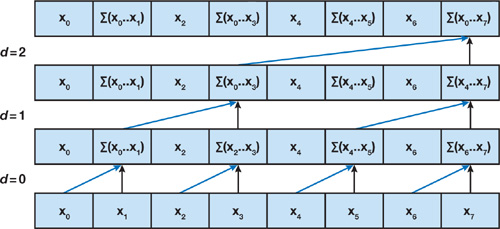
\includegraphics[width=0.6\textwidth]{scan_work_efficient_up_sweep}
\caption{The up-sweep phase of a work efficient parallel scan \cite{gpu_gems_3_chapter_39}}
\label{fig:scan_work_efficient_up_sweep}
\end{figure}

The first phase is called the reduce or up-sweep phase and is illustrated in figure \ref{fig:scan_work_efficient_up_sweep}. It takes an input array whose length must be a power of two. All elements of the input array are leaves of the tree. The algorithm than takes adjacent pairs of elements and adds them together forming a node holding the sum of it's two child nodes. This step forms a pass of the up-sweep phase and is repeated for the created parent nodes until the root of the tree which than holds the sum of all values. As the values of the right child nodes are not needed anymore after their parent nodes have been calculated, the tree can be built in-place.

\begin{figure}[h]
\centering
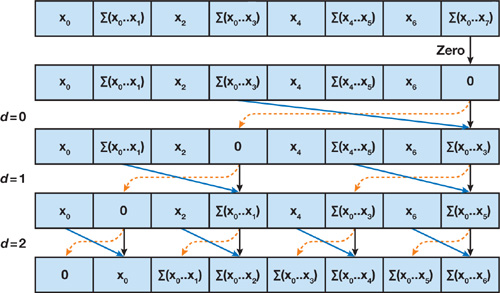
\includegraphics[width=0.6\linewidth]{scan_work_efficient_down_sweep}
\caption{The down-sweep phase of a work efficient parallel scan \cite{gpu_gems_3_chapter_39}}
\label{fig:scan_work_efficient_down_sweep}
\end{figure}

The second phase sets the value of the root node to zero to prepare for the third phase, the down-sweep phase, which is illustrated in figure \ref{fig:scan_work_efficient_down_sweep}. The down-sweep phase again consists of several passes starting at the root node and repeating along all levels of the tree until the leaves. In each pass the values of the left child nodes are read and temporarily stored. The left child nodes are than replaced by the value of their parent nodes. The previous, temporarily stored values of the left child nodes are then added to the parent nodes' values and written to the right child node. As the parent nodes are not needed anymore after the sum for the right child has been calculated, the tree can again be traversed downwards in-place.
Overall, for an input array of $n$ elements, this algorithm performs $n - 1$ adds during the up-sweep phase and the same amount of adds during the down-sweep phase\footnote{A perfect binary tree with $n$ leaves has a total of $2n - 1$ nodes. As only the non-leaf nodes perform additions, the number of leaf nodes can be subtracted resulting in $2n - 1 - n = n - 1$ nodes which perform an addition.}. Although almost twice as much work is performed when compared with the sequential CPU implementation, this algorithm can still be considered work-efficient according to the definition given in section \ref{sec:scan_cpu}.
Listing \ref{lst:scan_work_efficient_host} shows the host code implementing the work-efficient tree based approach after Blelloch \cite{scan_blelloch}.

\lstset{basicstyle=\ttfamily{}\scriptsize{}}
\lstinputlisting[language=CPP, caption=Host code for the work-efficient scan algorithm., label=lst:scan_work_efficient_host, firstline=66, lastline=103]{code/scan/main.cpp}
\lstset{basicstyle=\ttfamily{}}

Contrary to the previous algorithms, this implementation will use two kernels, one for the up-sweep and one for the down-sweep phase. 
To start with, the number of input elements has to be rounded up to be a power of two. This size is then used to create a buffer which is filled with the input array.
After these initialization steps we can begin with the up-sweep phase. The loop variable for the passes is the offset of the buffer index between two adjacent nodes on the same tree level. This value starts with one for the first pass and is raised to the next power of two for each subsequent pass until the size of the input buffer has been reached. For each pass the up-sweep kernel is enqueued with the buffer and the current pass' offset as arguments. The number of work items required for a pass is equal to the number of parent nodes calculated on the current pass' level. This value is a half of the buffer size for the first pass and halves itself after each pass. Although this algorithm is still independent of the chosen work group size, we have to make sure that it is not larger than the global number of work items. \\
After the up-sweep phase has been completed, the last element corresponding to the tree's root node will be set to zero. This is easily accomplished by enqueuing a write operation writing the value zero to the last buffer element. \\
Finally the down-sweep phase can finish the scan computation. Similar to the up-sweep phase several passes are executed given the offset between two adjacent tree nodes on the same level and the buffer as argument. In contrast to the up-sweep phase, the tree is now traversed top-down meaning the offset starts with a half of the buffer size and is set to the next lower power of two in each pass until one has been reached. Analogous, the number of nodes to process (the global work size) starts with one and doubles every pass.
When the down-sweep phase has completed, the buffer holds the final scan result which can than be read back to host memory.
Listing \ref{lst:scan_work_efficient_kernel} shows the corresponding OpenCL kernel code for the work-efficient scan implementation.

\lstset{basicstyle=\ttfamily{}\scriptsize{}}
\lstinputlisting[language=CL, caption=OpenCL Kernel code for the work efficient scan algorithm., label=lst:scan_work_efficient_kernel]{../src/scan/gpu/thesis/WorkEfficientScan.cl}
\lstset{basicstyle=\ttfamily{}}

The \lstinline!UpSweep! kernel starts by computing the value of \lstinline!stride! which is the distance of two parent nodes in the current pass. This value is used to calculate the buffer index (\lstinline!id!) of the current parent node (equal to the right child node) from the work items global id. The input value at \lstinline!id! is read (right child) together with the corresponding neighbor node at the given offset (left child). The computed sum is then written over the right child's location. \\
The \lstinline!DownSweep! kernel initializes the same way as it's preceding one by determining the current pass' stride and the parent node's index. Then, the value of the parent node is read and temporarily stored. The value of the left child node (given by \lstinline!offset!) is added the parent node (which becomes the right child node). Finally the previous, temporarily stored value of the parent node is passed down to the left child node.

When having a look at the benchmark results for this algorithm in figure \ref{fig:scan_chart} we can see that our efforts have payed off. The initial 1132 ms of the naive GPU implementation have shrunk to 604 ms on an array of $2^{26}$ elements. Furthermore, this implementation is now work-efficient and therefore avoiding unnecessary additions. Additionally, as all intermediate results are stored in-place, the algorithm does not waste memory by double buffering, such as the naive approach. However, the algorithm requires the input to be a power of two, which becomes more disadvantages with larger input sizes. %This can be clearly seen in the performance data table of the work-efficient scan in appendix section \ref{sec:scan_chart_data}, where the time required for the calculation is equal for all problem sizes that are round up to the same power of two. This also explains the stepped shape of the runtime curve.
This can be clearly seen at the stepped shape of the runtime curve which rises at every new power of two as the time required for the calculation is equal for all problem sizes that are round up to the same power of two.

\section{Recursively scanning blocks in local memory}
\label{sec:scan_recursive}

The previous work-efficient implementation in section \ref{sec:scan_work_efficient} does already perform quite well for an initially sequential problem. However, the input buffer size restriction is undesirable. Furthermore, no local memory is used which might be useful for computing and storing intermediate results.

\begin{figure}[h]
\centering
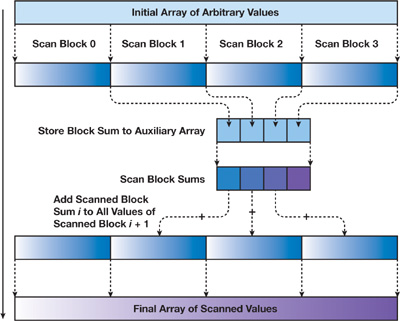
\includegraphics[width=0.5\linewidth]{scan_recursive}
\caption{Scanning larger arrays of values recursively \cite{gpu_gems_3_chapter_39}.}
\label{fig:scan_recursive}
\end{figure}

GPU Gems 3 Chapter 39 \cite{gpu_gems_3_chapter_39} shows a different approach for computing all prefix sums of an input array. The method is shown in figure \ref{fig:scan_recursive}. The input data is rounded up to be a multiple of a block size (which is two times the chosen work group size in their implementation). Each work group then loads a block from global memory to local memory. Each block is then scanned using Blelloch's work-efficient scan algorithm \cite{scan_blelloch}, but in local memory inside a work group. After the up-sweep phase is finished, the root element of each tree in a block is copied into a smaller, temporary buffer. This buffer is then recursively scanned again. The scan result of the temporary buffer can then be used to offset the scanned blocks of the original buffer to build the final scan.
Although this algorithm is not tied to a specific work group size it performs better the larger the work group size is chosen, as the work group sizes determines the factor by which the input data is reduced in each recursion.
Listing \ref{lst:scan_recursive_host} shows the host code of this recursive scan algorithm.

\lstset{basicstyle=\ttfamily{}\scriptsize{}}
\lstinputlisting[language=CPP, caption=Host code for the recursive scan algorithm., label=lst:scan_recursive_host, firstline=105, lastline=140]{code/scan/main.cpp}
\lstset{basicstyle=\ttfamily{}}

This implementation again uses two kernels, one for scanning the blocks in local memory and one for applying the offsets from the scanned temporary buffer to the original one. The host code consists of two parts, the setup code and the actual recursion. The setup is performed in \lstinline!recursiveGPU! which starts by rounding the input data size up to be a multiple of twice the size of a work group, because each work item processes two values. Then a buffer is created and the input data written to it. This buffer is then passed to the recursive scan procedure \lstinline!recursiveGPU_r!. The recursion starts by computing the size of the temporary buffer \lstinline!sums! that will hold the values of the root nodes (the sums over each block). As each thread processes two input elements and each work group computes one sum over a block, this temporary buffer's size is the problem size divided by two times the work group size. The result is then rounded up to be a multiple of this value, so it can be recursively scanned again with this algorithm. After the size has been determined, the \lstinline!sums! buffer can be created. No initialization or memory transfer is required as the buffer is entirely accessed by the kernels. Afterwards, the block scan kernel can be set up. It takes the original input buffer as well as the buffer for the sums as arguments. Furthermore local memory is allocated to cache the block calculated by each work group. As each work item reads two input elements, the global work size is half the number of input elements. After the kernel has been enqueued, we have to check whether the input data for this recursion consisted of more than one block. If this is the case we scan the temporary buffer (containing more than 1 value) by recursively calling \lstinline!recursiveGPU_r! on this buffer. After scanning the temporary \lstinline!sums! buffer has completed, the sums can be applied to the original buffer. Therefore another kernel is enqueued given both buffers as arguments. The global and local work size are equal to the previous kernel on the same recursion level.
Listing \ref{lst:scan_recursive_kernel} shows the kernel code for the recursive scan implementation.

\lstset{basicstyle=\ttfamily{}\scriptsize{}}
\lstinputlisting[language=CL, caption=OpenCL Kernel code for the recursive scan algorithm., label=lst:scan_recursive_kernel, firstline=1, lastline=55]{../src/scan/gpu/thesis/RecursiveScan.cl}
\lstset{basicstyle=\ttfamily{}}

The \lstinline!ScanBlocks! kernel starts with querying some values from OpenCL. Beside the global and local id, also the size \lstinline!n! of the block of the current work group is determined. Each thread than loads two values of the block into local memory. The following code then implements the tree based scan approach by Blelloch which has already been discussed in the previous section \ref{sec:scan_work_efficient}. The three phases (up-sweep, set-last-zero and down-sweep) are executed across all threads of the work group on the block in local memory. The only difference is, that the computed value of the root node after the up-sweep phase is moved to the \lstinline!sums! buffer at the index of the current work group. After the block has been scanned completely, it is copied back from local to global memory.

The \lstinline!AddSums! kernel is executed with the same global and local sizes as specified to the \lstinline!ScanBlocks! kernel on the same recursion level. The \lstinline!sums! buffer now contains a scan of the sums of all blocks scanned in this recursion. Therefore, the position where the \lstinline!ScanBlocks! kernel wrote the root node's value, now contains the sum of all elements (of all blocks) preceding the block of the current work group. This value is retrieved and added to all values of the current block finishing the scan.

Concerning the performance benchmark in figure \ref{fig:scan_chart}, this implementation scales better with the problem size although it is not faster than the global work-efficient scan of the previous section (606 vs. 604 ms on $2^{26} elements$). Furthermore, the recursive implementations' kernels are enqueued far less often than the one's of the work-efficient implementation. This can be explained by the reduction factor in each algorithm. The work efficient implementation reduces the number of work items by a factor of two each iteration while the recursive algorithm reduces by the work group size (which was 256 for the benchmarks) times two. In return, a lot more work is done inside the recursive algorithm's kernels. Also the number of additions required to compute the final result increased as extra adds a needed to apply the sums from the temporary buffer to the input buffer.
However, this implementation showed a different concept of how a problem can be broken down into smaller parallel pieces of work. The next implementation will follow up on this idea.

\section{Optimization using vector types}
\label{sec:scan_vector}

The final implementation shown in this chapter takes the idea of the recursive scan approach from the previous chapter one step further \cite[ch.39.2.5]{gpu_gems_3_chapter_39}. Instead of loading only two elements in each work item we will load two vectors of elements. These are then scanned inside each work item. The sums of the vectors (root node after the up-sweep phase) is then copied to local memory. The algorithm then continues just as the previous chapter's version by scanning the blocks in local memory. The results can then be used to offset the vectors of each work item just as the \lstinline!AddSums! kernel on a higher level. The remaining part of the implementation basically stays the same.
With this modification, each work group does not only load a block of two times the work group size of elements but a block of two times the work group size times the chosen vector width. As a result the input array is reduced faster by a factor of the chosen vector width in each recursion. The consumed local memory stays the same as only the sums of both vectors are placed into local memory. Only the consumed registers will increase.
Listing \ref{lst:scan_recursive_vector_host} shows the differences of the host code of the this vector type implementation compared with the previous one.

\lstset{basicstyle=\ttfamily{}\scriptsize{}}
\lstinputlisting[language=CPP, caption=Host code for the recursive scan algorithm using vector types., label=lst:scan_recursive_vector_host, firstline=143, lastline=152]{code/scan/main.cpp}
\lstset{basicstyle=\ttfamily{}}

The first and most important step is to define the width of the vectors used. OpenCL supports vector types with the lengths of 2, 4, 8 or 16. The larger this \lstinline!VECTOR_WIDTH! is chosen, the larger is the reduction of the input buffer in each recursion. However, as a side effect the consumed registers per work item increase leading to a lower occupancy of the kernel. The ideal vector width may be hardware specific and is subject to corresponding benchmarks. This implementation will use a \lstinline!VECTOR_WIDTH! of 8.
The remaining changes to the host code are straight forward. As the blocks get bigger by a factor of \lstinline!VECTOR_WIDTH!, the size of the temporary \lstinline!sums! buffer decreases by and has to be rounded up to the same factor. Furthermore, the global work size shrinks. Finally, the check whether the input array consisted of more than one block has to be adapted to the new block size.
Although the changes to the host code are quite small, the kernel needs a few more extensions as shown in listing \ref{lst:scan_recursive_vector_kernel}.

\lstset{basicstyle=\ttfamily{}\scriptsize{}}
\lstinputlisting[language=CL, caption=OpenCL Kernel code for the recursive scan algorithm using vector types with a width of eight., label=lst:scan_recursive_vector_kernel, firstline=156, lastline=234]{code/scan/main.cpp}
\lstset{basicstyle=\ttfamily{}}

First of all, several macros are defined for the \lstinline!ScanBlocksVec! kernel to avoid redundant code for the up-sweep and down-sweep implementation on the vector types. The kernel begins, after querying topological informations, by copying two \lstinline!int8! vectors into registers. The up-sweep phase is completely executed on the work item's registers on both vectors resulting in a lot of independent instructions. After the up-sweep phase, the last vector elements hold the sum over both vectors which is then copied into the shared memory block. After the last elements are reset to zero, the down-sweep phase continues, finalizing the scan on the two vectors stored in registers. The remaining part of the kernel is equal to the one of the previous implementation in listing \ref{lst:scan_recursive_kernel} which calculates the scan of the block in shared memory and copies the block's sum into the \lstinline!sums! buffer. A final small addition is to offset the vectors by the sum of all previous vectors of preceding work items in this block. Notice that the value loaded from local memory is added to each vector element. Finally the vectors are written back to global memory. \\
The \lstinline!AddSums! kernel only changes by the type of the buffer which now consists of \lstinline!int8!s. Also notice here, that the value of \lstinline!val! loaded from the \lstinline!sums! is added to all vector elements of the two vector elements of \lstinline!buffer!.

When having a look at the benchmark results in figure \ref{fig:scan_chart} we can clearly see a difference to the previous, non-vector implementation. The 604 ms of the non-vector implementation could be reduced by 37\% to 383 ms for a problem size of $2^{26}$ input elements. This is already an amazing result for a sequential problem such as scan. Nevertheless, the initial CPU scan time of 225 ms is still out of reach.
%However, if we have a closer look at the benchmark data in appendix section \ref{sec:scan_chart_data} we might notice that the final recursive vector scan implementation actually beat the CPU implementation when it comes down to run time. 
However, if one has a closer look at the benchmark data one can see that the final recursive vector scan implementation actually beat the CPU implementation when it comes down to run time. It took only 87 ms to scan the $2^{26}$ elements on the GPU. Upload and download have the larger shares of the total time required of the GPU scan, contributing 154 and 141 ms for transferring the 256 MiB to and from the GPU's main memory. This means that 77 \% of the total run time is wasted on memory transfers, which is a huge problem for many memory intensive algorithms like scan. Figure \ref{fig:scan_mem_transfer_chart} shows a detailed view on the upload, run and download phase of the recursive vector scan implementation.

\begin{figure}[h]
\centering
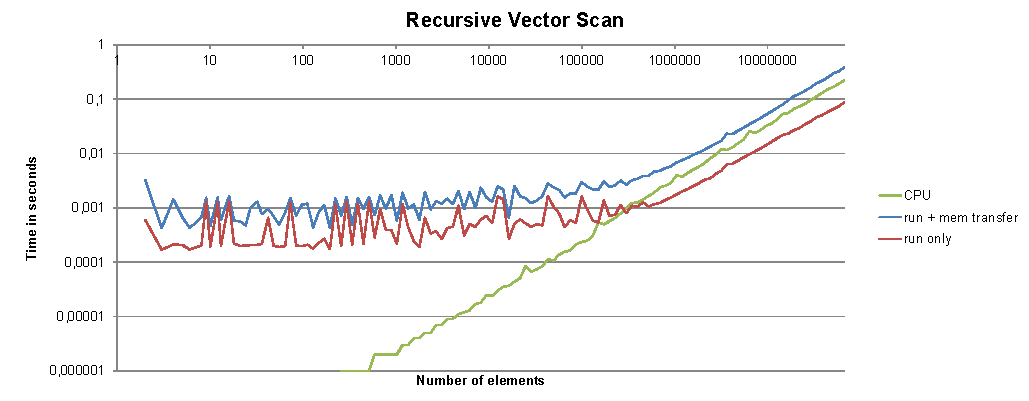
\includegraphics[width=1.0\linewidth]{scan_vector_chart}
\caption{A closer look to the benchmark of the recursive vector scan from section \ref{sec:scan_vector}. It points out how much time is wasted by memory transfers.
%The chart is based on the benchmark data in appendix section \ref{sec:scan_chart_data}.
Note that both axis are of logarithmic scale. }
\label{fig:scan_mem_transfer_chart}
\end{figure}

\section{Further implementations}
Beside the presented kernels a further approach has been implemented and benchmarked which has not been covered. However some experiences may help future developers.

\begin{description}
	\item[Bank conflict avoidance] \hfill \\
	The GPU Gems 3 chapter about scan \cite{gpu_gems_3_chapter_39} also talks about avoiding bank conflicts occurring in the kernel in chapter \ref{sec:scan_work_efficient} where blocks are scanned in local memory. Both recursive scan implementations (chapters \ref{sec:scan_recursive} and \ref{sec:scan_vector}) have been implemented using the presented approach to avoid bank conflicts. However, the time required to calculate the conflict free offsets to local memory compensates for the time won by faster local memory access.
\end{description}

Furthermore, several libraries exist supporting GPGPU accelerated scans.

\begin{description}
   \item[clpp \cite{clpp}] \hfill \\
   The OpenCL Data Parallel Primitives Library is an open source and freely available library offering a few GPU primitives such as a scan and sort implementation. However, the project seems to be inactive (last release in July 2011).
   \item[ArrayFire \cite{arrayfire}] \hfill \\
   ArrayFire is a commercial GPU software acceleration library provided by AccelerEyes. It provides a lot of GPGPU accelerated algorithms using CUDA and OpenCL including scan.
%   \item[Apple \cite{apple_scan}] \hfill \\
%   Apple provides an example implementation of a parallel prefix sum using OpenCL in their Mac Developer Library.
%   \item[AMD \cite{amd_app_sdk}] \hfill \\
%   AMD also provides an example implementation of scan as part of their APP SDK.
%   \item[NVIDIA \cite{nvidia_opencl_samples}] \hfill \\
%   Finally, scan is also part of NVIDIA's OpenCL example codes which can be downloaded from their website.
\end{description}

\section{Summary and conclusion}
In this chapter we have seen how a sequential algorithm like the all-prefix-sum can be parallelized for GPUs. A tree based approach using several passes delivered good results. Also the idea of solving the problem in smaller sub groups which are than merged into the global result proofed to be successful. Both concepts are common patterns when trying to port sequential CPU code to a GPU. However, we did also learn that using a GPU does not always result in a performance boost, despite their enormous power. So does the final scan only perform three times faster than the CPU implementation excluding memory transfer. If the time for copying the data to and from the GPU's main memory is included, we would be better off staying with the CPU. This is a problem for many fast algorithms operating on larger chunks of memory. Nevertheless, a fast GPU implementation of such primitives can still be needed in cases where the input and output data is already present or consumed on the GPU. This is the case when input data is produced on the GPU (e.g., scanning image data from a rendering process) or present as input for other purposes (other algorithms, data for rendering). Also the output may be directly used by the GPU (e.g using scan as part of a filtering routine generating a list of objects to render). Even if a GPU algorithm would be slower in run time than a CPU version it might still outperform the CPU variant including memory transfer to and from the systems main memory.


\chapter{Sorting}
\label{sec:sorting}

One of the most fundamental operations in computer science is sorting a sequence of elements. And as old as the problem is, as numerous are the algorithms to solve it. These sorting algorithms differ in various aspects such as best, average and worst runtime or memory complexity, stability, the number of comparisons and swaps and whether the algorithm is a comparison based sort or not.

The sort implementations provided by today's standard libraries are highly tuned and achieve an optimal asymptotic runtime complexity of $\mathcal{O}(n\:log\,n)$ for comparison based sorts. Examples are variations of quick sort (C), merge sort (C++), intro sort (C++, .NET) or Timsort (Java, Python). All these algorithms are comparison based sorts, thus requiring a method of comparing two elements of the input sequence. This comparison is often provided either by the language or standard library (e.g., $<$ operator) or by the programmer via a custom comparison function, giving the flexibility to compare and sort any kind of elements.

Another class of sorting methods are integer sorting algorithms. These algorithms do not use comparisons to determine the order of elements. They rely on more flexible integer arithmetic applied to the keys which have to be sorted. Therefore, they have a better asymptotic runtime complexity than comparison based ones. Popular algorithms of this kind are radix sort, counting sort and bucket sort. All of them running with $\mathcal{O}(n + k)$ or $\mathcal{O}(n * k)$ (where $k$ is a constant) in linear time.
However, despite their limitation on the sort key, integer sorting algorithms also work on other kind of types as long as they can be represented as integers in binary (e.g., strings can be seen as byte array forming a (larger) integer).

Considering parallelizability and an eventual GPU implementation, sorting lies between matrix multiplication and prefix sum offering some degree of parallelism depending on the chosen algorithm. This chapter will focus on the implementation of two widely chosen algorithms for GPU sorting. These are the comparison based bitonic sorting network and the integer sorting algorithm radix sort. To reduce code complexity (especially of the latter), the input array consists of unsigned 32 bit integers.

\begin{figure}[!p]
\centering
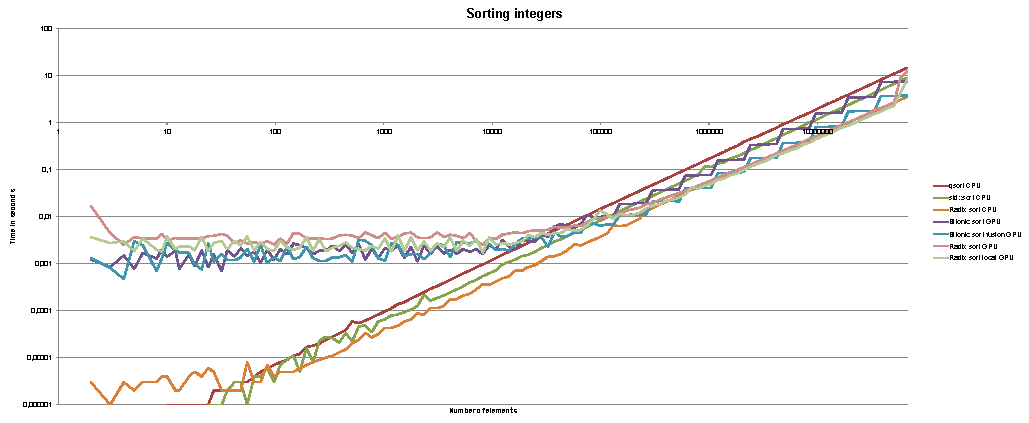
\includegraphics[width=0.9\textheight, angle=90]{sort_chart}
\caption{Benchmark of several sort implementations.
%The chart is based on the benchmark data in appendix section \ref{sec:sort_chart_data}.
Both axis are of logarithmic scale. Integer sorting algorithms (radix sort) are drawn in dashed lines.}
\label{fig:sort_chart}
\end{figure}

\section{CPU Implementations}

Before stepping into the details of the two chosen GPU algorithms, bitonic and radix sort, a set of CPU sorting algorithms is discussed. Their resulting run times are used as a reference and compared with the GPU implementations in the benchmarks.

\pagebreak

\subsection{C/C++ standard library routines}

As the later GPU implementations should be compared with well implemented and wide-spread CPU ones, the first step is to measure the performance of the standard library's routines.
Listing \ref{lst:sort_cpu_qsort} shows a typical usage of the \lstinline!qsort! function provided by the stdlib header from C.

\lstset{basicstyle=\ttfamily{}\scriptsize{}}
\lstinputlisting[language=CPP, caption={Sorting an array of unsigned integers using \lstinline!qsort! from the C stdlib header. The provided comparison lambda function uses comparisons instead of simply subtracting the input values (\lstinline!a - b!) as this may cause unwanted behaviour due to overflows (e.g., \lstinline!1u - MAX_UINT! is $2$ instead of a negative number). Subtraction does work for signed types.}, label=lst:sort_cpu_qsort, firstline=34, lastline=44]{code/sort/main.cpp}
\lstset{basicstyle=\ttfamily{}}

As \lstinline|qsort| is usually precompiled and part of the runtime library, a compare function has to be provided which is called for every comparison. This will probably slow down the run time when compared with the C++ \lstinline!std::sort! which can use an existing overload of the $<$ operator or inline a provided compare function.
Listing \ref{lst:sort_cpu_sort} shows a typical call to the \lstinline!std::sort! function template from the C++ algorithm header.

\lstset{basicstyle=\ttfamily{}\scriptsize{}}
\lstinputlisting[language=CPP, caption={Sorting an array of unsigned integers using \lstinline!std::sort! from the C++ algorithm header.}, label=lst:sort_cpu_sort, firstline=46, lastline=48]{code/sort/main.cpp}
\lstset{basicstyle=\ttfamily{}}

As the $<$ operator is defined for unsigned integer types no custom compare function has to be provided and no additional overhead is created for comparing elements.
The difference in the benchmark chart in figure \ref{fig:sort_chart} is evident. It takes \lstinline!qsort! 14.746 seconds to sort a sequence of $2^{26}$ elements while \lstinline!std::sort! only requires 9.039 seconds.

\subsection{Radix sort}
\label{sec:sorting_radix_cpu}

In contrast to the comparison based \lstinline!qsort! and \lstinline!std::sort!, radix sort operates on the binary representation of the input elements in several passes. The input values are therefore seen as numbers of a numeral system of a chosen base (= radix). In each pass, a digit at the same position (starting with the least significant) is selected from all input elements. These input elements are then split into buckets according to the value of the current pass' digit. Elements with the same digit value retain their order.

If the radix is two, in each pass a bit (digit) of each input element (number represented in the binary system) is selected (starting with the least significant bit). The input elements are then split into two sequences (buckets) according to the selected bit. This is done by creating a histogram holding the number of elements having the same bit value for each bit combination (0 or 1). After the histogram has been created, it is exclusively scanned. The scanned histogram now holds the start index for each bucket. The input elements are permuted and moved into their corresponding buckets according to the selected bit. Elements with an equal bit are written into the same bucket in the same order as they appeared in the pass' input (each pass is stable). An auxiliary array is usually needed for this permutation step. This procedure is repeated for every bit of the input elements. 

\pagebreak

By only selecting one bit in each pass, 32 passes are required to sort the input sequence (elements are 32 bit unsigned integers). In each pass the input array is iterated over two times and the histogram has to be scanned once. This accumulates to 64 iterations over the input sequence and 32 scans of a two element histogram making radix sort a linear algorithm but with a quite significant constant factor. This factor can be reduced by selecting several bits of each input element at once in each pass (increasing the radix to a larger power of two). As a result, the number of passes decreases linearly with the number of selected bits (which is called radix and gives the algorithm its name). As a trade-off, the size of the histogram increases by a power of two.
The CPU radix sort implementation used in the benchmarks is provided in listing \ref{lst:sort_cpu_radix}.

\lstset{basicstyle=\ttfamily{}\scriptsize{}}
\lstinputlisting[language=CPP, caption=Sorting an array of unsigned integers using radix sort. The algorithm uses two passes analyzing 16 bits each. The implementation is based on the radix sort sample shipped with AMD APP SDK \cite{amd_app_sdk}., label=lst:sort_cpu_radix, firstline=50, lastline=93]{code/sort/main.cpp}
\lstset{basicstyle=\ttfamily{}}

The implementation uses a relatively high radix of 16 (\lstinline!RADIX!) which allows radix sort to finish in two passes. As a consequence, the histogram consists of $2^{16}$ elements (\lstinline!BUCKETS!) occupying 256 KiB of memory but has to be scanned only two times.

The performance difference of radix sort to the previously presented comparison based algorithm is significant as seen in figure \ref{fig:sort_chart}. Although the high radix of 16 causes a large overhead on small input sizes (as the full $2^{16}$ element histogram has to be scanned independently of the input size), radix sort shows its strength on larger inputs. It catches up to \lstinline!std::sort! at approximately 10,000 elements and then outperforms the library routine largely sorting $2^{26}$ elements in 0.884 seconds (compared to 9.039 seconds of \lstinline!std::sort!).

\section{GPU Implementations}

After the presented CPU sorting routines in the previous sections, the following sections focus on creating efficient bitonic and radix sorting implementations for the GPU using OpenCL.

\subsection{Bitonic Sort}

Many regular sorting algorithms do not fit into a GPU's massively parallel programming model by offering insufficient parallelism, requiring non-array data structures or begin based on recursion. However, a small subgroup of sorting approaches exists that fits the requirements of parallel hardware perfectly: sorting networks. A sorting network is a network of wires (one for each input) and comparators along these wires. Comparators connect two wires, compare their values and might swap them.
Finding optimal sorting networks for a given number of inputs is difficult and still subject to research. However, in 1968 Ken Batcher presented (beside others) an approach to create sorting networks achieving reasonable results \cite{sort_bitonic}. His idea is based on efficiently merging a bitonic sequence into a sorted sequence, hence the name bitonic sorter. A bitonic sequence is a sequence of elements which consists of two equally long subsequences, where one is sorted ascending and the other descending. As two arbitrary elements form a bitonic sequence, they can be merged into a sorted sequence. As two sequences sorted in opposite order also form a bitonic sequence they can again be merged into a sorted sequence. This allows us to create sorting networks for any power of two sized inputs.

\begin{figure}[h]
\centering
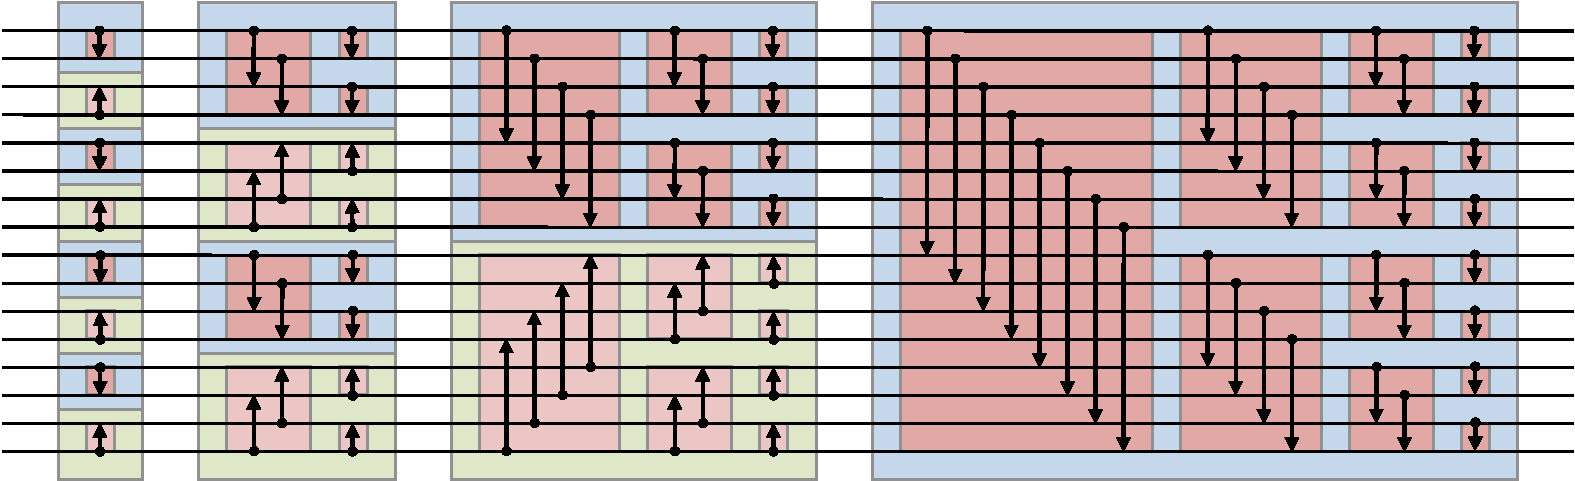
\includegraphics[width=0.8\linewidth]{bitonic_sort}
\caption{Example of a bitonic sorting network for 16 inputs \cite{wiki_bitonic_sort}.}
\label{fig:bitonic_sort}
\end{figure}

Figure \ref{fig:bitonic_sort} shows a bitonic sorting network for 16 input elements. The input elements start on the left side of the network and travel through it to the right. Each arrow represents a comparator which compares the elements of the connected wires and swaps them if necessary, so that the larger element is swapped to the wire the arrow points at. Each blue or green box is a separate bitonic merge receiving a bitonic sequence as input and outputting a sorted one (blue = ascending, green = descending). The red boxes contain the comparators and are equally structured. They compare the top half of the input (bitonic) sequence against the bottom half and create two bitonic sequences where each element of the upper bitonic sequence is smaller than or equal to every element in the bottom one (vice versa in green boxes). Further red boxes are than recursively applied to the two outputs until the sequence is sorted.

The created networks consist of $\mathcal{O}(n\:log^2\,n)$ comparators. As $\frac{n}{2}$ comparators can be executed in parallel (cf. figure \ref{fig:bitonic_sort}), the runtime complexity of a bitonic sorter would be $\mathcal{O}(log^2\, n)$ on a computer with at least $\frac{n}{2}$ processing elements.

Sorting inputs of any length is also possible with a bitonic sorting network. The network is constructed for the next larger power of two and all comparators affecting a wire of a (possible) input element larger than the actual input are omitted. This approach and a sample implementation is discussed in more detail in an online article by Hans Lang \cite{sort_bitonic_arbitrary_n}. To keep the code simple, the bitonic sorter implementation presented in this chapter will only focus on inputs with a power of two length.
Listing \ref{lst:sort_bitonic_host} shows the host code of a bitonic sorter implementation.

\lstset{basicstyle=\ttfamily{}\scriptsize{}}
\lstinputlisting[language=CPP, caption=Host code for a bitonic sort implementation. \cite{sort_bealto}., label=lst:sort_bitonic_host, firstline=95, lastline=123]{code/sort/main.cpp}
\lstset{basicstyle=\ttfamily{}}

At first the input's size is rounded up to a power of two (\lstinline!adjustedSize!). A read- and writable buffer is created with this size and the input data is written to it. If the input was smaller than the created buffer, the remaining part is filled with the maximum representable value of the input data type. This values should remain at the back side of the buffer during the sorting procedure and not disturb the actual input. As sorting networks are compare-and-swap-based no additional buffer is required. The input can be sorted in place.
After the buffer is set up we can begin sorting the elements.

As we can see in figure \ref{fig:bitonic_sort}, each column of red boxes contains half as many comparisons as inputs, which can be executed in parallel. Therefore, a kernel will be enqueued for every column of red boxes consisting of $\frac{n}{2}$ work items. The distance between two wires of a comparator is equal across all red boxes of a column and will be called \lstinline!inc!. The red boxes itself are combined in colums of alternating blue and green boxes. The width of these boxes (the number of wires they span) will be called \lstinline!boxWidth! and determines the initial \lstinline!inc! (which is a half of the width) of their contained columns of red boxes. Furthermore, the \lstinline!boxWidth! allows each comparator to derive the sorting direction (ascending or descending) from the wires'/work items' indexes.

The approach is implemented using two nested loops. The outer loop iterates the \lstinline!boxWidth!s which are powers of two (starting with two) until the last blue box, which is equally long to the number of inputs. The inner loop iterates over the distances between two wires of the comparators inside the red box columns (\lstinline!inc!). This value starts with a half of the \lstinline!boxWidth! and decreases to the next lower power of two each loop until one.
In each iteration of the inner loop a kernel is enqueued. Arguments are the inner loops \lstinline!inc!, the other loops \lstinline!boxWidth! and the buffer with the values. The global work size is the number of comparisons of the current red box column which is a half of the input size. The local work size can be chosen freely except it must not be larger than the global one.
After all passes have been executed, the sorted values can be read back from device memory.
Listing \ref{lst:sort_bitonic_kernel} shows the corresponding kernel code for the described bitonic sorter implementation.

\pagebreak

\lstset{basicstyle=\ttfamily{}\scriptsize{}}
\lstinputlisting[language=CL, caption=OpenCL Kernel code for one iteration of a bitonic sort. The implementation is based on an article about experiences with OpenCL and sorting by Eric Bainville \cite{sort_bealto}. , label=lst:sort_bitonic_kernel,]{../src/sort/gpu/thesis/BitonicSort.cl}
\lstset{basicstyle=\ttfamily{}}

The kernel begins by calculating the index of the first wire for the comparator corresponding to the current work item. This is achieved by modifying the global id. The bits below the \lstinline!inc! bit (the lower part) stay the same. This value determines the wire index in the upper half of a red box. The bit at position \lstinline!inc! of the global id corresponds to the upper (0) or lower (1) half of the red box. This bit shall be zero to get the upper wire of the comparator. The remaining (upper) part of the global id above the \lstinline!inc! bit is a multiple of the width of a red box and therefore determines the index of the red box inside the column. As only $\frac{n}{2}$ work items have been enqueued, the upper part has to be doubled to have box indexes for the full range of wires. The combined value is stored in \lstinline!i!.
The next step is to decide upon the sorting order of the current comparator. This can be done by looking at the bit at position \lstinline!boxWidth! of the upper wire's index. If this bit is zero, the comparator belongs to a blue box and the sorting order is ascending. Otherwise we are in a green box and have to sort descending.
Afterwards the two values at the input wires of the comparator are loaded from global memory. The positions are \lstinline!i! and \lstinline!i + inc!. If the values have to be swapped they are written back to global memory in opposite order.

Looking at the performance data in figure \ref{fig:sort_chart} we can see that the GPU bitonic sorter performs equally well as C++'s \lstinline!std::sort!. If we look very closely we can even see that the bitonic sorter's runtime raises a bit faster than the one of the CPU sorting algorithm. This can be explained simply by their runtime complexities which are $\mathcal{O}(n\: log^2\,n)$ for the bitonic network and $\mathcal{O}(n\:log\,n)$ for \lstinline!std::sort!.
When profiling the code the first problem that can be noticed are the number of enqueued kernels, which is 1053 for an input of $2^{26}$ elements. Furthermore, the large number of work items are quite lightweight. The latter is not a problem as such but it is important to notice that here is still space for optimization. Fortunately, both issues can be solved by combining several separate kernel invocations into a larger, heavier kernel. This is also known as kernel fusion and topic of the next section.


\subsection{Bitonic Sort using kernel fusion}

The basic concept of kernel fusion is to reduce the amount of redundant global memory loads and stores to the same locations between two or more separate kernel invocations.
Using the example of the bitonic sorting network for 16 inputs in figure \ref{fig:bitonic_sort}, kernel fusion could be used to combine the kernel invocations for the second and third column of red boxes. Considering only the upper blue box, work item zero and one would load the values of wire zero to three. After the first red box all four values would be stored back to global memory. On the next kernel invocation, work item zero and one would again load the same values for the following two red boxes of the same column. By combining the two separate kernel invocations into one, the redundant global memory store and load between the two kernels could be avoided.
This idea can be taken further to combine even more invocations into a single kernel. However, fusing kernels tends to making the work items heavier in resource consumption. Considering the bitonic sorting network where each work item initially had to store two values from global memory, the fused kernel (combining two invocations) would require storing four values per work item (and reducing the global work size to $\frac{n}{4}$). This value increases by powers of two and therefore sets a limit to the amount of kernels that can be fused together.
Listing \ref{lst:sort_bitonic_fusion_host} shows the changes to the previous bitonic sorter host implementation.

\lstset{basicstyle=\ttfamily{}\scriptsize{}}
\lstinputlisting[language=CPP, caption=Changes to the host code from listing \ref{lst:sort_bitonic_host} for a bitonic sort implementation using kernel fusion. \cite{sort_bealto}., label=lst:sort_bitonic_fusion_host, firstline=125, lastline=173]{code/sort/main.cpp}
\lstset{basicstyle=\ttfamily{}}

The outer and inner loop enqueuing the kernels stay the same. However, if the increment \lstinline!inc! is large enough a fused kernel can be used which processes more than one column of red boxes with multiple increments (decreasing powers of two). The largest fused kernel being used is \lstinline!kernel16! which processes 16 input values and fuses four invocations with four different increments. Larger kernels are still possible, but showed to consume to much registers to increase performance (register spilling). Nevertheless, larger kernels may be beneficial on newer hardware with more available registers. By using \lstinline!kernel16! the inner loop's \lstinline!inc! variable can be incremented to the fourth lower power of two instead of the next one, which is controlled by the \lstinline!ninc! variable. Kernels with eight, four and two inputs follow analogously. The kernel with two inputs is actually the original one used before kernel fusion.
After the appropriate kernel has been chosen it is enqueued with the same parameters as an unfused kernel. Only the number of enqueued work items decreases as each work item now processes more values.
The corresponding kernel code is based on the previous section in listing \ref{lst:sort_bitonic_kernel}. As several very similar kernels have to be created, the preprocessor is used to reduce redundant code.

\pagebreak

\lstset{basicstyle=\ttfamily{}\scriptsize{}}
\lstinputlisting[language=CL, caption={OpenCL code of several (fused) kernels performing 1, 2, 3 or 4 iterations (2, 4, 8 or 16 inputs per work item) of a bitonic sort. \cite{sort_bealto}.} , label=lst:sort_bitonic_fusion_kernel,]{../src/sort/gpu/thesis/BitonicSortFusion.cl}
\lstset{basicstyle=\ttfamily{}}

The kernel code starts with the \lstinline!order! procedure which orders two values (at index \lstinline!a! and \lstinline!b!) of a given array \lstinline!x! either ascending or descending depending on the value of \lstinline!asc!. The following \lstinline!BITONIC_SORT_FUSION! macro declares the actual kernel plus a merge procedure. Arguments to the macro are the number of input wires the expanded kernel should process (\lstinline!lvl!) as well as the logarithm of base two for this value (\lstinline!logLvl!). Finally also the half of the \lstinline!lvl! argument has to be specified. This value cannot be calculated as it is used in token pasting and macro expansion.

The macro begins by declaring a merge procedure for the current number of input wires. Arguments are a pointer to the array holding the values of the input wires (\lstinline!x!) and a boolean determining the sort order (\lstinline!asc!). For the half number of input wires, comparison have to be made (cf. a larger red box in figure \ref{fig:bitonic_sort}). Then both halves of the input array are merged using two invocations of the merge procedure of the next lower level (half the current input wires). This is the actual fused part of the kernel which now processes the next two smaller red boxes sharing the same inputs as the initial red box. Although the merge procedure is recursive, it cannot be implemented as such due to OpenCL not allowing recursive function calls. The reason for this is that OpenCL programs do not have a runtime stack for storing local (not \lstinline!__local!!) variables. They have to be stored in registers and therefore the maximum amount of necessary register space needed by the program has to be determinable at compile time (and will be fully allocated when the kernel is executed). The final \lstinline!merge2! procedure will not have to call any recursive merges any more. Therefore the macro \lstinline!merge1! is declared empty (recursion anchor).

After the merge procedur the actual kernel for \lstinline!lvl! number of inputs follows. The code is basically taken from the previous, non-fused version from the last section. The first adjustment made is to decrease the kernel's increment to the one of  the last fused original kernel's invocation. Furthermore, when constructing the wire index of the first value to load, not only the bit at \lstinline!inc!'s position is set to zero but \lstinline!logLvl! bits, as \lstinline!lvl! values will be loaded instead of two. These values are loaded from global memory starting at the computed index \lstinline!i! with a stride of \lstinline!inc!. The core forms the invocation of the bitonic merge on the loaded array\footnote{As the loaded values of the input wires have to be simply sorted, it is possible to replace the bitonic merge by any kind of sorting algorithm.}. The sorted values are then written back to global memory.
Finally the macro is expanded to produce a merge procedure and a kernel for the levels 2, 4, 8 and 16.

The difference in performance can be seen clearly when comparing the fused bitonic sorter against the previous implementation in figure \ref{fig:sort_chart}. For sorting $2^{26}$ elements the fused variant only requires 3.808 seconds which is roughly two times faster than the original version (7.678 seconds). This is mostly due to reduced global memory traffic by cutting down the number of enqueued kernels which has shrunken to 294 (compared with the initial 1053). In comparison to \lstinline!std::sort!, which requires 9.039 seconds, this is a speedup of 2.37.

The implementation can still be improved by taking advantage of local memory. Eric Bainville also shows a version of the fused level four kernel using local memory in his excellent article from which most of this bitonic sort approaches are taken from \cite{sort_bealto}. The benchmarks however only show an insignificant boost (several milliseconds) in performance on the cost of a relatively complex kernel. Therefore this idea will not be covered.

Another idea would be to place the loaded values from the wires into local memory as local memory is accessible on a 4-byte boundary (1-byte with OpenCL extension cl\_khr\_byte\_addressable\_store). Arrays in registers can only by accessed by index at full register boundaries (16 byte) forcing the compiler to allocate more register space than the initial array requires. By placing arrays in local memory the register usage of work items could be cut down allowing higher occupancy on the cost of slower memory access. With a work group size of 256 (used in all benchmarks and the maximum of the used GPU), a level 32 kernel would already consume the full 32 KiB of local memory on the used GPU. However, when placing the array in registers, a level 32 kernel would already spill registers into global memory which is incredibly slow. Therefore a level 32 kernel might be beneficial when using local memory. Nevertheless, this approach has not been tested with the bitonic sorter. This idea is reconsidered when discussing radix sort in section \ref{sec:sorting_radix_local}.


\subsection{Radix Sort}
\label{sec:sorting_radix}

We have already discussed radix sort in the CPU implementation section \ref{sec:sorting_radix_cpu}. Implementing radix sort for the GPU comes down again to three steps which are executed in passes. The first step is to create a histogram for the radix of the current pass. Secondly, the histogram has to be scanned and finally, the input values are permuted according to the scanned histogram.

Creating the histogram would be easy. For each input element a work item is created which determines the histogram element (bucket) which should be incremented. By using atomic operations which are available since OpenCL 1.1 (extension in OpenCL 1.0) the histogram can simply be stored in global memory and concurrently updated from all threads without errors. As global memory atomics are relatively slow, each work group should first compute a histogram in local memory which is then finally reduced to one in global memory.

However, this kind of histogram is of little to no use during the fully parallel permute stage. The reason for this is that every work item must be able to determine the destination address for its value independently of other threads. Although it would be possible for all work items of the same histogram bucket to obtain different destination addresses again by using atomic increments on the histogram (similar to the CPU implementation where each bucket's histogram value is incremented after writing a value to this bucket), it does not work on a GPU. Because OpenCL does not guarantee the order in which work items are executed, work items with higher global id might write values to a bucket before work items with lower id do. As a consequence the permute pass would not be stable anymore which is crucial to not ruin the permutation of a previous pass.

A solution to this problem can be found by thinking about the information a work item needs to find its correct destination address. In addition to the the start address of the region where all values of the same bucket should be written to (as in a single histogram), each work item also needs to know how many work items having a value belonging to the same bucket have a smaller global id than the current work item. This can be solved by spreading the histogram down to all individual work items. As each work item now owns a separate histogram memory consumption raises enormously. Therefore, multiple input values are processed in each work item. The histograms, after they have been created by the work items, are moved to global memory as such that the histogram entries of the same bucket across all work items lie consecutively and ascendingly (concerning the global id) in memory followed by the next group of buckets and so forth. As a result, the scan step can simply scan the whole block of histogram memory without any special cases. Therefore, the vector scan kernel developed in section \ref{sec:scan_vector} can be fully reused as building block for this radix sort implementation. 
Listing \ref{lst:sort_radix_host} shows the host code for an OpenCL radix sort implementation.

\lstset{basicstyle=\ttfamily{}\scriptsize{}}
\lstinputlisting[language=CPP, caption=Host code for a radix sort implementation. \cite{amd_app_sdk}., label=lst:sort_radix_host, firstline=204, lastline=259]{code/sort/main.cpp}
\lstset{basicstyle=\ttfamily{}}

\pagebreak

At the top of the source code several macros define constants. The first three should already be known from the previous CPU implementation in section \ref{sec:sorting_radix_cpu}. A major difference is the relatively small radix used with the GPU implementation. This is justified by the huge amount of memory required to store a histogram of $2^{RADIX}$ buckets for each work item. New is the \lstinline!BLOCK_SIZE! constant which defines how many elements each work item processes. Its value of 32 has been determined by benchmarks and may be specific to the used GPU. The \lstinline!VECTOR_WIDTH! macro defines the width of the vector types used in the scan kernel (cf. vector scan implementation in chapter \ref{sec:scan_vector}). 
The host code stars by creating two buffers with the size of the input rounded up to be a multiple of the work group size times the \lstinline!BLOCK_SIZE!. One will be used to hold the input values at the beginning of each pass (source) and the other one will be used by the permute step to write the output values to (destination). The source buffer is initialized with the unsorted input sequence from host memory. Any free space after the written sequence is filled up with the largest representable value of the input elements' data type.
Beside the source and destination buffer a further histogram buffer is needed to store a histogram for each work item. The size of this buffer has to be rounded up to fit the input size requirements for the vector scan. 
The global work size is the number of input elements divided by \lstinline!BLOCK_SIZE! as each work item processes \lstinline!BLOCK_SIZE! values. The local work size can be chosen at will as the algorithm does not depend on local memory or work group synchronization.
After the setup is complete we can start executing several sort passes identically to the CPU variant. In each pass a histogram kernel is enqueued which calculates the per work item histograms and stores them into the histogram buffer. Arguments of the kernel are the source buffer containing the input values, the histogram buffer for writing the histograms to and the bit offset of the current pass to select the corresponding bits of the input keys. After the histograms are created and stored in global memory, the histogram buffer can be scanned. The vector scan algorithm (host and kernel) from section \ref{sec:scan_vector} will be used directly for this job. The scanned histograms are then input to the permute kernel which will reorder the values from the source buffer into the destination buffer. Finally the references to the source and destination buffer are swapped for the next pass.
After all passes have been executed the resulting sorted sequence can be read from the source buffer (destination buffer of the last pass).
Listing \ref{lst:sort_radix_kernel} shows the corresponding kernel code.

\lstset{basicstyle=\ttfamily{}\scriptsize{}}
\lstinputlisting[language=CL, caption={OpenCL code for the histogram and permute kernels of a radix sort, where each work item stores it's histogram in registers. \cite{amd_app_sdk}} , label=lst:sort_radix_kernel, lastline=34]{../src/sort/gpu/thesis/RadixSort.cl}
\lstset{basicstyle=\ttfamily{}}

The \lstinline!Histogram! kernel begins by querying the global id of the work item and setting up a zero initialized array for holding the histogram values. Each work item then processes \lstinline!BLOCK_SIZE! elements of the input buffer. For each element the bits corresponding to the current pass' bit offset are extracted to increment the appropriate bucket of the work item's histogram. After processing the input elements has finished, the histogram is split into its buckets and moved to global memory. \\
The \lstinline!Permute! kernel begins with copying the scanned histogram back from global memory into registers. Each histogram bucket now contains the number of elements belonging into this bucket from work items with lower global id plus the sum of all elements of preceding buckets. Then the work item again reads in the \lstinline!BLOCK_SIZE! input elements for which the scanned histogram is now available. Each value is written to the destination buffer at the start address of the corresponding bucket for this work item. The address is incremented afterwards.

Considering performance (cf. figure \ref{fig:sort_chart}), the radix sort GPU implementation is roughly equally fast as the fused bitonic sort. When looked closely, one can even see that radix sort's runtime increases a little bit slower than the one of the bitonic sorter. However, the GPU radix sort cuts off at the last few input sizes as the GPUs global memory is exhausted and the driver starts to swap GPU memory into the systems main memory. Nevertheless, the GPU implementation is far behind the CPU variant with 1.884 seconds at $2^{25}$ (!) elements compared to 0.449 seconds on the CPU.
When profiling the kernel one can see that most of the time is spent executing and waiting for global memory requests. If we have a look at the kernel code in listing \ref{lst:sort_radix_kernel} again, we can see that the \lstinline!Histogram! kernel performs \lstinline!BLOCK_SIZE! read operations of four byte (size of uint). Furthermore adjacent work items access global memory with a stride of \lstinline!BLOCK_SIZE! times four byte. As a result each four byte value from each work item is loaded using a full memory transaction. However, on NVIDIA GPUs memory transactions always load a full memory segment of 64 or 128 words (32-bit values) \cite[p.13]{nvidia_opencl_best_practices}. Global memory access should therefore be coalesced, meaning that adjacent work items should access adjacent elements in global memory. In this case, all work items can be serviced in as few memory transactions as possible. However, this is not possible in our radix sort implementation unless the \lstinline!BLOCK_SIZE! is reduced to one. Nevertheless, another way of increasing memory bandwidth utilization is to request fewer but larger pieces of memory. This approach also improves performance on AMD GPUs and will be covered in section \ref{sec:sorting_radix_local_vec}.
A further but more subtle issue can be seen in the disassembly of both kernels. The local (not \lstinline!__local!) array \lstinline!uint hist[BUCKETS]! is placed in a work item's registers. However, a register's size is four words (equal to an \lstinline!uint4!). To allow indexing the array (runtime indexing into registers is not possible), the array has to be either placed strided into registers (each array element occupies only the first component of each vector register) or the compiler has to generate appropriate code to transform an index into the corresponding register address and vector component. An unorthodox but working solution is to put the array into shared memory which can be addressed at a 4-byte boundary (1-byte with OpenCL extension cl\_khr\_byte\_addressable\_store). This idea will be covered in the following section.

\subsection{Radix Sort using local memory}
\label{sec:sorting_radix_local}

Instead of placing each work item's histogram in it's own registers, local memory is used to store the array. Thus, wasted register space and instruction overhead necessary to access an array placed in registers is avoided. However, accessing local memory is usually slower and accesses might suffer from bank conflicts. This implementation will take the radix sort of the previous section \ref{sec:sorting_radix} and move the histogram from registers to local memory.
Listing \ref{lst:sort_radix_local_host} shows the required changes to the host code from listing \ref{lst:sort_radix_host}.

\lstset{basicstyle=\ttfamily{}\scriptsize{}}
\lstinputlisting[language=CPP, caption=Changes to the host code of listing \ref{lst:sort_radix_host} for a radix sort implementation using local memory to store each thread's histogram. \cite{amd_app_sdk}., label=lst:sort_radix_local_host, firstline=306, lastline=312]{code/sort/main.cpp}
\lstset{basicstyle=\ttfamily{}}

As local memory is shared inside a work group, we have to allocate a block of local memory large enough to hold all histograms of all work items of a work group. The local memory needs to be allocated in both kernels.
Listing \ref{lst:sort_radix_local_kernel} shows the required changes to the kernel code from listing \ref{lst:sort_radix_kernel}.

\lstset{basicstyle=\ttfamily{}\scriptsize{}}
\lstinputlisting[language=CL, caption=Changes to the OpenCL kernel code of listing \ref{lst:sort_radix_kernel} for a radix sort implementation using local memory to store each thread's histogram. \cite{amd_app_sdk}, label=lst:sort_radix_local_kernel, firstline=312, lastline=334]{code/sort/main.cpp}
\lstset{basicstyle=\ttfamily{}}

Instead of declaring \lstinline!hist! as local variable inside the kernel, it is now passed as pointer to \lstinline!__local! memory as an argument to both kernels. The pointer has then to be offsetted to the current work item's histogram place. Except initialization to zero in the \lstinline!Histogram! kernel, the remaining code stays the same.

Benchmarking the changed code shows a subtle but noticeable difference in performance. The initial 1.884 seconds of the original implementation from section \ref{sec:sorting_radix} could be reduced to 1.565 seconds, simply adjusting the code to fit better to the GPUs hardware features. Although this code has executed faster in the benchmarks, newer GPUs might already provide scalar registers having no troubles storing an array of scalar data types.

\subsection{Radix Sort using local memory and vector loads}
\label{sec:sorting_radix_local_vec}

A further optimization of the presented radix sort implementation is to replace the many small global memory reads in both radix sort kernels by fewer but larger fetches. This can be achieved by declaring the pointers to the input buffers in both kernels to be of a vector type. Therefore the number of iterations of the fetching loops (and therefore the number of fetches) is reduced by a factor of the width of the used vector type. Disadvantages of using vector types may be increased register consumption and increased source code length (vector components cannot be iterated over).
As this only concerns the kernel itself, no changes to the host code are required. Listing \ref{lst:sort_radix_local_vec_kernel} shows the changes to the previous radix sort implementation using local memory from listing \ref{lst:sort_radix_local_kernel}.

\lstset{basicstyle=\ttfamily{}\scriptsize{}}
\lstinputlisting[language=CL, caption=Changes to the OpenCL kernel code of listing \ref{lst:sort_radix_local_kernel} for a radix sort implementation using local memory to store each thread's histogram and vector types for loading values from global memory. \cite{amd_app_sdk}, label=lst:sort_radix_local_vec_kernel, firstline=338, lastline=371]{code/sort/main.cpp}
\lstset{basicstyle=\ttfamily{}}

The first difference is the increase of the \lstinline!BLOCK_SIZE! constant which was 32 and has been raised to 128. It turned out that the larger memory requests now impose a smaller problem concerning the total runtime. Thus, more of them can be made inside each work item (may be specific to a GPU and should therefore be tested individually). To maximize memory throughput the largest supported vector type is chosen for the input buffer which is \lstinline!uint16!. As a result the fetching loops only need to iterate over a 16th of \lstinline!BLOCK_SIZE! input elements. The number of required iterations is placed in the macro \lstinline!BLOCK_SIZE_16!. In each loop iteration a full \lstinline!uint16! (64 byte) value is fetched from global memory and the target bucket in the histogram is calculated. Now comes the drawback of using vector types. As we cannot loop over the components of the fetched value, we have to write code for each histogram access using a different component separately.

When we look at the benchmark chart in figure \ref{fig:sort_chart} we can see that our effort paid off. Compared with the version without vector fetches we could achieve a speedup of 1.5 (1.019 vs. 1.565 seconds). Beside a far better memory bus utilization also the amount of independent instruction increased leading to better ALU utilization.
However, despite the optimizations, the GPU radix sort implementation runs still slower than the original CPU code. Reasons are the slow global memory write accesses in both radix sort kernels and the relatively small \lstinline!RADIX! of four compared to 16 in the CPU variant which leads to eight passes on the GPU compared to only two on the CPU.


\section{Further implementations}
Beside the presented kernels a further approach has been implemented and benchmarked which has not been covered. However some experiences may help future developers.

\begin{description}
	\item[Odd-Even Transition \cite{gpu_gems_2_chapter_46}] \hfill \\
	The odd-even transition sorting network from gpu gems 2 chapter 46 \cite{gpu_gems_2_chapter_46} has been implemented. However, performance was significantly worse than the other covered algorithms.
\end{description}

Furthermore, several libraries exist supporting GPGPU accelerated sorting routines.

\begin{description}
	\item[clpp \cite{clpp}] \hfill \\
	The OpenCL Data Parallel Primitives Library is an open source and freely available library offering a few GPU primitives such as a scan and sort implementation. However, the project seems to be inactive (last release in July 2011).
	\item[libCL \cite{libCL}] \hfill \\
	libCL is an open-source library with the intention to provide a variety of all kinds of parallel algorithms. Although the list of functions is still small, it provides an implementation of radix sort.
	\item[ArrayFire \cite{arrayfire}] \hfill \\
	ArrayFire is a commercial GPU software acceleration library provided by AccelerEyes. It provides a lot of GPGPU accelerated algorithms using CUDA and OpenCL including a sorting routine.
%	\item[AMD \cite{amd_app_sdk}] \hfill \\
%	AMD also provides an example implementation of radix sort as part of their APP SDK. The presented implementations in this section are based upon the one by AMD. Furthermore, also a bitonic sort can be found.
%	\item[NVIDIA \cite{nvidia_opencl_samples}] \hfill \\
%	Finally, radix and bitonic sort are also part of NVIDIA's OpenCL example codes which can be downloaded from their website.
\end{description}

\section{Summary and conclusion}
Sorting an array of elements is one of the most used routines of a programmer. Numerous algorithms and libraries (also standard libraries) exist targeting the CPU and providing highly optimized and ready-to-use sorting routines. However, the availability of GPU accelerated routines is still limited and mainly consists of some experimental libraries. In this chapter we have seen how to implement both, a comparison based and an integer based sorting algorithm using OpenCL. Contrary to traditional concepts, sorting networks where introduced offering a higher amount of parallelism on the cost of runtime complexity. The bitonic sorter has been discussed as example of how a sorting network can be constructed and operated for a given input size. Kernel fusion has been presented as a further way of optimizing algorithms consisting of multiple OpenCL kernels or kernel invocations. Radix sort has been introduced as example of a fast integer based sorting routine. Beside noticing the bad handling of arrays in registers, the final radix sort implementation once again showed the importance of global memory utilization.
In conclusion, a fast comparison based sorting routine could be presented beating C++'s \lstinline!std::sort! with a speedup of 2.37 (9.039 vs. 3.808 seconds on $2^{26}$ elements). Unfortunately, radix sorting is still faster on the CPU with the OpenCL implementation being more than twice as slow as the simple C++ variant.


\chapter{Conclusion}
\label{sec:conclusion}

\section{Summary}

OpenCL is a free and open standard for general purpose parallel programming across various hardware devices. It is maintained by the Khronos Group and implemented by hardware vendors like NVIDIA, AMD or Intel. OpenCL is natively available for C and C++ although many wrappers for other languages exist. To use OpenCL in a C/C++ application an SDK is needed which contains the required header files (also available from Khronos) and static libraries. For running an application using OpenCL a corresponding driver has to be installed offering the API functions as well as a compiler to create kernels. Furthermore, one or more appropriate hardware devices supporting OpenCL are necessary and may even be used together.

The hardware architectures for which OpenCL can be used are quite different, especially concerning the differences between CPUs and GPUs.
Modern consumer CPUs have a small number of independent, high power cores (mostly four or eight) which can be used independently by an application using threads. Synchronization between the threads is easy and threads may be spawned at any time. High throughput can be achieved by distributing the work on all available cores and make use of vector instruction sets like SSE or AVX. Memory is provided as a large block behind a hierarchical cache system.

GPUs however employ a massive amount of less powerful cores (up to several thousands) packed together in multiprocessors. Work is processed in smaller work groups and larger n-dimensional ranges which often occupy hundreds or thousands of threads (which often have to be a multiple of hardware specific resources) executing the same code step by step. Synchronization is limited and the amount of threads used has to be predetermined every time work is offloaded to the GPU. High throughput is achieved by utilizing all components of the GPU (ALU, read and write units, etc.) as much as possible. Branching and synchronization should be avoided and vector types/operations should be used wherever possible to maximize the ALUs throughput. The large global memory is cached but very slow and sensitive concerning access patterns. Local memory is available as programmers-controlled cache but again suffers from misaligned accesses (bank conflicts). However, GPUs can achieve a much higher computational throughput than CPUs when used correctly.

Using OpenCL in an application starts by choosing an available platform/implementation and device. Additionally, a context and a command queue have to be created. Kernels are mostly created directly from their source code which has to be provided at run time. The source code is then compiled and linked into a program for the selected device and the kernels can be queried by name. To provide larger input and to retrieve output from a kernel, buffer objects have to be created. These may be read from and written to, either asynchronously or synchronously to the main application, by enqueuing operations on the command queue. Kernels are also enqueued and executed asynchronously after their arguments have been set.

To show the strengths and weaknesses of OpenCL and GPGPU computing on a few real world examples, three kinds of problems have been chosen for which various approaches have been implemented and benchmarked.

\begin{enumerate}
	\item
	At the beginning, multiplying two square matrices was ported to OpenCL. The CPU implementation is trivial but performs badly. Fortunately, highly tuned BLAS libraries exist which can do the multiplication a lot faster on the CPU. However, the first and again quite simple OpenCL implementation already beats the efficient BLAS sgemm routine. With some optimizations, making the code more complicated, we could push performance even further, achieving a speedup of 36.
	By the example of matrix multiplication we also took a look into performance analysis using profiler information from AMD's CodeXL.
	
	\item
	The second problem tackled was the all-prefix sum, a linear algorithm. The CPU implementation can be coded in a minute using a simple loop in a few lines of code. A naive, also quite easy to understand GPU approach performed fairly poor. By trying a more sophisticated tree-based reduce and scatter algorithm, small improvements could be made. Adding local memory and finally also using vector types and applying the algorithm on several layers in the end showed significant cut-downs on the run time (at the cost of hundreds of lines of code). However, the runtime of the CPU could not be beaten.
	
	\item
	The last implementation chapter focused one of the most famous topics in computer science, sorting. The two standard library routines \lstinline!qsort! and \lstinline!std::sort! have been benchmarked together with a radix sort implementation, the latter delivering amazing results. For sorting on the GPU, sorting networks have been introduced, because they are easy to parallelize. In particular, the bitonic sorter has been implemented and optimized. Despite the nasty input size restriction, the GPU implementation runs more than twice as fast as the comparison based variants on the CPU, which can be clearly seen as success. Radix sort, however, suffers from the GPUs highly parallel nature. Despite several optimizations it could not catch up and remains far behind the CPU implementation.
\end{enumerate}


\section{Conclusion}

In conclusion it can be said that GPUs are different from CPUs in the way they process work. This originates from their quite dissimilar hardware architectures as we discussed in the beginning. But not only the hardware itself, also the way algorithms have to be designed and programs have to be written differs largely from traditional single-thread-orientated CPU algorithms. Although it is already quite common to assign several tasks to several CPU cores (e.g., GUI and work thread), bringing parallelism down to small routines is still far from being common. When a program is designed to be run on massively parallel hardware we tend to spend more time on fighting with the peculiarities of the hardware than thinking about the actual problem we try to solve. This was one of the hardest challenges when implementing scan. The scan operation imposes high data dependency between the processed elements and therefore makes it perfectly suitable for as few processing units as possible. The GPU however benefits from a maximum of parallelism, on data and instruction level. Most of the time required to develop an efficient GPU scan was spent on trying to get enough parallelism on the cost of minimal redundancy in additions. Although the tree based approach worked well in the end, a lot of computing power is wasted during the up-sweep and down-sweep phase inside each work group. The same problem affected the radix sort GPU implementation. The per work item histogram was only required because the GPU does not ensure the order in which work items are processed. And to improve memory reading performance for the scan step by aligning the histogram buffer for coalesced access, the scattered, unblocked writes of the histograms at the end of the permute step also teared down performance, because GPUs profit enormously from reading and writing larger, consecutive blocks of memory. On the CPU, apart from worse caching, scattered accesses is less of a problem. The final argument, that should arise from this observations, is that programmers have to worry about a lot more different stuff than they have to when coding for a processor. Imagine Java or C\# programmers who are used to object-oriented design, dynamic memory allocation, huge standard libraries, containers and other complex data structures and all that candy of modern languages, when they find themselves porting one of their well-written, readable algorithms to the GPU where they have to break everything down into well-layouted arrays, think about the vectorizability of the produced instructions, repeatedly check the API documentation for a small number of built-in functions that might be of use and hunt down performance issues to stalled memory reads and bank conflicts. GPGPU computing is far different from modern software design and programming. Although the API is easily understood and the kernel language quickly learned, it takes months and probably years of practice to get a good feeling for designing GPU accelerated algorithms. GPUs are technological marvels offering immense computational power if used correctly. But it takes time to learn and study them in order to unfold their full potential.

Furthermore, it has to be said that not all algorithms fit the requirements of a GPU. In fact, only a small subset really benefits from the massively parallel hardware. In most cases, it is easier to focus on spreading a workload on several cores of the CPU instead of dealing with thousands of threads. Also the required memory transfer to and from the GPU is a crucial factor when deciding to offload a piece of work or not. If an algorithm does not fit the GPU one should not execute it there.

However, the small subset of algorithms which is often parallel in its nature may benefit tremendously from graphics hardware. We have discussed such a kind of algorithm on the example of multiplying matrices. The final speedup of 36 is amazing and shows the potential of GPU hardware when used at the right place.

So, when should OpenCL be used? Apart from having the right kind of algorithm to take advantage of GPGPU acceleration, also time and budget play an important role. Developing an algorithm for the GPU can be tedious and cumbersome and therefore time consuming. Furthermore, GPUs also impose a higher risk of failing to achieve the desired performance boost. The scan algorithms with optimizations may have taken two weeks to develop with the final outcome that the CPU variant is still faster. Experimenting with GPUs in a real world project should therefore be considered well, also concerning the aspect of system requirements. From a developers perspective, appropriate GPUs have to be available for implementing and testing and additional tools have to be installed for debugging and profiling. Concerning customers, appropriate hardware has to be available, drivers have to be installed and maybe the case of missing compatible hardware or drivers has to be handled (fallback CPU implementation). Talking about tools, the currently available suits from AMD (CodeXL), NVIDIA (Nsight, Visual Profiler) and Intel (SDK for OpenCL Applications) already provide decent help when developing software for their respective GPUs. However, they are still quite away from being as suitable and feature-rich as corresponding CPU debugger integration and profilers. Last but not least also maintainability and reusability play a vital role in modern software companies. Both aspects suffer in most cases as OpenCL algorithms tend to be optimized strongly to a specific kind of hardware and problem.

Finally, we have to see how long GPGPU computing will be done in this fashion. With the increasing power of on-chip GPUs on modern Intel processors, using GPUs for smaller tasks might become more attractive as no memory transfers will be required. AMD is also working intensively on a new generation of processing devices called Accelerated Processing Units (APU). By using a so-called heterogeneous system architecture (HSA), GPU and CPU are combined tightly on a single chip. The GPU will have direct access to the system's main memory with cache coherence to the CPU using the same address space as the CPU (theoretically allowing pointers to be passed). Furthermore, the GPU will allow multitasking via context switches between running tasks. As a result, long-running calculations will no longer freeze the display.
However, in another corner of the high performance hardware sector, Intel is heavily working on their new Many Integrated Core (MIC) architecture. The Intel Xeon Phi (previously named Knights Corner) is a co-processor card with up to 61 individual Intel processors and up to 16 GiB dedicated on-card memory. From an OpenCL programmers perspective, the Xeon Phi is equally programmed as a GPU. But the card is composed of modified x86 processors and can therefore also execute conventional software written in traditional languages. As a result, language integration is also easy. In fact, Intel's compiler already offers appropriate \lstinline!#pragma!s to offload parts of a C++ program to the co-processor card in a similar fashion as OpenMP. In addition, almost all drawbacks of GPUs vanish as all threads (four cores on each processor) can be fully synchronized, memory can be allocated dynamically on demand and all existing language features including libraries can be used. However, a Xeon Phi is still financially out of reach for consumers and still more expensive than decent GPUs with prices among several thousand dollars. But as time passes by, they may become affordable. Intel already announced that the next generation of the Xeon Phi (codename Knights Landing) will be capable of being used as the systems main processor. So maybe in ten years we find ourselves with a hundred main processors in our notebooks capable of handling even computationally expensive software with ease. Who needs GPU computing then?

\section{Experiences}

asasdf

\addcontentsline{toc}{section}{List of figures}
\renewcommand\listfigurename{List of figures}
\listoffigures

\clearpage

\addcontentsline{toc}{section}{List of listings}
\renewcommand\lstlistlistingname{List of listings} 
\lstlistoflistings

\clearpage

\addcontentsline{toc}{section}{References}
%\appto{\bibsetup}{\emergencystretch=1em}
\setcounter{biburllcpenalty}{9000}
\printbibliography[title=References]

\appendix
\section{Appendix}

\subsection{Matrix multiplication chart data}
\label{sec:matrix_mul_chart_data}

\subsubsection{Naive CPU}

\begin{tabular}{r r r}
size & run time mean & run time deviation \\
1 & 0 & 0 \\
25 & 0,000018 & 0 \\
50 & 0,000149 & 0,000019 \\
75 & 0,000524 & 0,000031 \\
100 & 0,001227 & 0,000156 \\
200 & 0,009001 & 0,000352 \\
300 & 0,035097 & 0,000099 \\
400 & 0,081693 & 0,000048 \\
500 & 0,198807 & 0,00369 \\
600 & 0,446807 & 0,022159 \\
700 & 0,885177 & 0,195293 \\
800 & 3,404683 & 0,063133 \\
900 & 6,094824 & 0,095358 \\
1000 & 9,158203 & 0,067449 \\
1100 & 12,273643 & 0,255862 \\
1200 & 16,473761 & 0,053628 \\
1300 & 20,301222 & 0,243348 \\
1400 & 25,209266 & 0,313975 \\
1500 & 30,550882 & 0,005375 \\
1600 & 39,762075 & 0,066254 \\
1700 & 44,930466 & 0,283708 \\
1800 & 54,965556 & 0,720861 \\
1900 & 61,130207 & 0,186277 \\
2000 & 74,531188 & 0,211783 \\
2100 & 83,185726 & 0,294925 \\
2200 & 96,555736 & 0,011703 \\
2300 & 110,60543 & 0,085392 \\
2400 & 133,480428 & 0,092403 \\
2500 & 142,234335 & 0,241012 \\
2600 & 161,313258 & 0,166381 \\
2700 & 181,084228 & 0,426846 \\
2800 & 210,357538 & 1,604625 \\
2900 & 229,775846 & 0,104415 \\
3000 & 263,874226 & 0,146529 \\
3100 & 286,894302 & 1,15429 \\
3200 & 314,497279 & 0,93643 \\
3300 & 345,02634 & 0,804373 \\
3400 & 397,331989 & 0,157337 \\
3500 & 436,245888 & 1,077226 \\
3600 & 488,217435 & 1,013651 \\
3700 & 525,113808 & 1,147087 \\
3800 & 560,915371 & 12,134538 \\
3900 & 624,880278 & 0,970673 \\
4000 & 657,499788 & 7,276395 \\
\end{tabular}

\subsubsection{OpenMP CPU}

\begin{tabular}{r r r}
size & run time mean & run time deviation \\
1 & 0,000201 & 0,000243 \\
25 & 0,000038 & 0,000001 \\
50 & 0,000124 & 0,000024 \\
75 & 0,000337 & 0,000039 \\
100 & 0,000679 & 0,000004 \\
200 & 0,006593 & 0,00036 \\
300 & 0,025074 & 0,000875 \\
400 & 0,065272 & 0,003128 \\
500 & 0,12838 & 0,002369 \\
600 & 0,464459 & 0,011541 \\
700 & 0,863346 & 0,0978 \\
800 & 1,776675 & 0,058818 \\
900 & 2,920025 & 0,047825 \\
1000 & 4,292602 & 0,02397 \\
1100 & 5,779423 & 0,032466 \\
1200 & 7,612406 & 0,08626 \\
1300 & 9,696026 & 0,027816 \\
1400 & 12,134429 & 0,055001 \\
1500 & 15,762018 & 0,196349 \\
1600 & 19,813159 & 0,294983 \\
1700 & 22,466314 & 0,229691 \\
1800 & 26,122541 & 0,089804 \\
1900 & 30,893081 & 0,208651 \\
2000 & 36,715405 & 0,271032 \\
2100 & 42,121322 & 0,025874 \\
2200 & 48,680537 & 0,143346 \\
2300 & 57,262861 & 0,705831 \\
2400 & 64,834907 & 0,097273 \\
2500 & 73,534766 & 0,18417 \\
2600 & 82,970566 & 0,135356 \\
2700 & 93,526126 & 0,38893 \\
2800 & 104,260969 & 0,467199 \\
2900 & 117,205018 & 0,35524 \\
3000 & 130,497517 & 0,991553 \\
3100 & 144,324302 & 1,200542 \\
3200 & 168,570176 & 1,039508 \\
3300 & 175,129977 & 0,230182 \\
3400 & 195,68473 & 1,115665 \\
3500 & 214,542733 & 0,94702 \\
3600 & 236,730639 & 0,425485 \\
3700 & 258,485694 & 0,532694 \\
3800 & 277,081415 & 1,662909 \\
3900 & 302,396295 & 0,657581 \\
4000 & 323,586431 & 2,265068 \\
\end{tabular}

\subsubsection{CBLAS CPU}

\begin{tabular}{r r r}
size & run time mean & run time deviation \\
1 & 0,000005 & 0,000007 \\
25 & 0,00001 & 0 \\
50 & 0,000059 & 0 \\
75 & 0,000192 & 0,000001 \\
100 & 0,00039 & 0,000003 \\
200 & 0,003063 & 0,000137 \\
300 & 0,012551 & 0,000072 \\
400 & 0,029367 & 0,000024 \\
500 & 0,056781 & 0,000061 \\
600 & 0,099672 & 0,001023 \\
700 & 0,201223 & 0,051646 \\
800 & 0,333364 & 0,086883 \\
900 & 0,456633 & 0,025736 \\
1000 & 0,678157 & 0,026632 \\
1100 & 0,887394 & 0,017413 \\
1200 & 1,219493 & 0,05202 \\
1300 & 1,494735 & 0,022683 \\
1400 & 1,896388 & 0,04717 \\
1500 & 2,315734 & 0,037512 \\
1600 & 2,858037 & 0,031083 \\
1700 & 3,508918 & 0,094538 \\
1800 & 4,086062 & 0,051909 \\
1900 & 4,806106 & 0,097737 \\
2000 & 5,62859 & 0,066646 \\
2100 & 6,078531 & 0,005372 \\
2200 & 6,998793 & 0,008354 \\
2300 & 8,031067 & 0,034976 \\
2400 & 9,107732 & 0,014117 \\
2500 & 10,299053 & 0,021374 \\
2600 & 11,575173 & 0,004663 \\
2700 & 12,983403 & 0,07307 \\
2800 & 14,490919 & 0,084496 \\
2900 & 16,092239 & 0,040324 \\
3000 & 17,804858 & 0,024317 \\
3100 & 19,637134 & 0,017677 \\
3200 & 21,580045 & 0,037946 \\
3300 & 23,737392 & 0,07079 \\
3400 & 25,977898 & 0,012364 \\
3500 & 28,343538 & 0,042341 \\
3600 & 31,180217 & 0,113045 \\
3700 & 33,803832 & 0,033084 \\
3800 & 37,478187 & 0,154286 \\
3900 & 39,98611 & 0,102763 \\
4000 & 43,48911 & 0,097813 \\
\end{tabular}

\subsubsection{Naive GPU}

\begin{tabular}{r r r r r r r r r}
size & upload time mean  & upload time deviation & run time mean & run time deviation & download time mean & download time deviation & wg size & up run down sum \\
1 & 0,00088 & 0,000671 & 0,000615 & 0,000291 & 0,000515 & 0,000098 & 16 & 0,002011 \\
25 & 0,002313 & 0,001245 & 0,001516 & 0,000214 & 0,001091 & 0,000138 & 16 & 0,00492 \\
50 & 0,000605 & 0,000246 & 0,000515 & 0,000122 & 0,000537 & 0,000069 & 16 & 0,001656 \\
75 & 0,001388 & 0,001341 & 0,000616 & 0,000189 & 0,000544 & 0,00006 & 16 & 0,002547 \\
100 & 0,000791 & 0,000289 & 0,000668 & 0,000095 & 0,000509 & 0,000021 & 16 & 0,001967 \\
200 & 0,000966 & 0,000187 & 0,002478 & 0,000078 & 0,000755 & 0,000027 & 16 & 0,0042 \\
300 & 0,00111 & 0,000203 & 0,006948 & 0,000004 & 0,00081 & 0,000043 & 16 & 0,008867 \\
400 & 0,001459 & 0,000156 & 0,015373 & 0,00003 & 0,000997 & 0,000004 & 16 & 0,017829 \\
500 & 0,001692 & 0,000255 & 0,0295 & 0,000057 & 0,001021 & 0,000054 & 16 & 0,032213 \\
600 & 0,002086 & 0,000095 & 0,049811 & 0,000103 & 0,001417 & 0,000168 & 16 & 0,053314 \\
700 & 0,002627 & 0,000152 & 0,078352 & 0,000156 & 0,001593 & 0,000111 & 16 & 0,082571 \\
800 & 0,003309 & 0,000287 & 0,116651 & 0,00038 & 0,002011 & 0,000312 & 16 & 0,121971 \\
900 & 0,003735 & 0,000176 & 0,166536 & 0,000032 & 0,002247 & 0,00034 & 16 & 0,172518 \\
1000 & 0,004558 & 0,000344 & 0,226959 & 0,000215 & 0,002512 & 0,000296 & 16 & 0,234028 \\
1100 & 0,005154 & 0,000159 & 0,300857 & 0,000079 & 0,00294 & 0,000401 & 16 & 0,308951 \\
1200 & 0,006172 & 0,000451 & 0,390213 & 0,000503 & 0,003762 & 0,00116 & 16 & 0,400147 \\
1300 & 0,007018 & 0,000246 & 0,498331 & 0,00018 & 0,003791 & 0,000678 & 16 & 0,50914 \\
1400 & 0,007851 & 0,000166 & 0,619719 & 0,000168 & 0,004264 & 0,000638 & 16 & 0,631833 \\
1500 & 0,00894 & 0,000164 & 0,760697 & 0,000259 & 0,004787 & 0,000716 & 16 & 0,774423 \\
1600 & 0,010071 & 0,000208 & 0,922575 & 0,000214 & 0,00528 & 0,000799 & 16 & 0,937926 \\
1700 & 0,011411 & 0,000169 & 1,110858 & 0,000437 & 0,00588 & 0,000912 & 16 & 1,128149 \\
1800 & 0,012665 & 0,000253 & 1,314582 & 0,000277 & 0,006421 & 0,001081 & 16 & 1,333667 \\
1900 & 0,013955 & 0,00022 & 1,543945 & 0,000435 & 0,007093 & 0,001145 & 16 & 1,564993 \\
2000 & 0,015383 & 0,00025 & 1,800036 & 0,000517 & 0,007745 & 0,001241 & 16 & 1,823163 \\
2100 & 0,018453 & 0,001132 & 2,089494 & 0,000709 & 0,00891 & 0,001781 & 16 & 2,116857 \\
2200 & 0,020629 & 0,001056 & 2,396777 & 0,00101 & 0,009662 & 0,001862 & 16 & 2,427068 \\
2300 & 0,021557 & 0,001121 & 2,73565 & 0,000838 & 0,010521 & 0,002003 & 16 & 2,767727 \\
2400 & 0,023792 & 0,001303 & 3,108474 & 0,00053 & 0,012114 & 0,002304 & 16 & 3,14438 \\
2500 & 0,025764 & 0,000829 & 3,525107 & 0,001671 & 0,013198 & 0,003711 & 16 & 3,564069 \\
2600 & 0,030394 & 0,003931 & 3,95678 & 0,000505 & 0,013523 & 0,002903 & 16 & 4,000697 \\
2700 & 0,02907 & 0,001087 & 4,425657 & 0,000171 & 0,014466 & 0,003151 & 16 & 4,469194 \\
2800 & 0,031051 & 0,001214 & 4,935096 & 0,000193 & 0,015604 & 0,00332 & 16 & 4,981752 \\
2900 & 0,034663 & 0,000787 & 5,499003 & 0,000063 & 0,018825 & 0,002719 & 16 & 5,55249 \\
3000 & 0,03674 & 0,000772 & 6,076687 & 0,000326 & 0,019522 & 0,002762 & 16 & 6,132948 \\
3100 & 0,039193 & 0,000626 & 6,699122 & 0,000248 & 0,020904 & 0,002895 & 16 & 6,759219 \\
3200 & 0,042414 & 0,000287 & 7,366433 & 0,000382 & 0,02241 & 0,003427 & 16 & 7,431257 \\
3300 & 0,044612 & 0,000872 & 8,098219 & 0,000295 & 0,023677 & 0,003526 & 16 & 8,166509 \\
3400 & 0,047597 & 0,000858 & 8,845134 & 0,001031 & 0,02558 & 0,003803 & 16 & 8,918311 \\
3500 & 0,05071 & 0,000831 & 9,642507 & 0,000035 & 0,026813 & 0,00355 & 16 & 9,720029 \\
3600 & 0,054842 & 0,000794 & 10,488255 & 0,000327 & 0,028352 & 0,003967 & 16 & 10,571449 \\
3700 & 0,05736 & 0,001358 & 11,412625 & 0,000414 & 0,031272 & 0,00441 & 16 & 11,501257 \\
3800 & 0,06071 & 0,001305 & 12,344899 & 0,000137 & 0,031608 & 0,004524 & 16 & 12,437216 \\
3900 & 0,064896 & 0,001158 & 13,335906 & 0,000247 & 0,033453 & 0,004929 & 16 & 13,434255 \\
4000 & 0,068064 & 0,001656 & 14,3872 & 0,000152 & 0,035069 & 0,00478 & 16 & 14,490333 \\
\end{tabular}

\subsubsection{Tiles GPU}

\begin{tabular}{r r r r r r r r r}
size & upload time mean  & upload time deviation & run time mean & run time deviation & download time mean & download time deviation & wg size & up run down sum \\
1 & 0,002448 & 0,001914 & 0,000439 & 0,0003 & 0,000479 & 0,000025 & 16 & 0,003365 \\
25 & 0,001442 & 0,000625 & 0,000323 & 0,000064 & 0,000495 & 0,000073 & 16 & 0,00226 \\
50 & 0,00142 & 0,000421 & 0,00036 & 0,000063 & 0,000495 & 0,000036 & 16 & 0,002275 \\
75 & 0,00147 & 0,000174 & 0,000391 & 0,000076 & 0,000528 & 0,00005 & 16 & 0,002389 \\
100 & 0,002443 & 0,001676 & 0,000485 & 0,000116 & 0,00057 & 0,000092 & 16 & 0,003498 \\
200 & 0,001545 & 0,000168 & 0,001096 & 0,000081 & 0,000638 & 0,000008 & 16 & 0,003278 \\
300 & 0,001548 & 0,000208 & 0,002783 & 0,000163 & 0,00069 & 0,000017 & 16 & 0,005022 \\
400 & 0,001627 & 0,000374 & 0,006297 & 0,000704 & 0,0007 & 0,000027 & 16 & 0,008624 \\
500 & 0,004134 & 0,000871 & 0,012672 & 0,000636 & 0,001544 & 0,000655 & 16 & 0,01835 \\
600 & 0,004918 & 0,003085 & 0,02007 & 0,000656 & 0,001241 & 0,000179 & 16 & 0,026228 \\
700 & 0,004176 & 0,000242 & 0,03017 & 0,000284 & 0,001945 & 0,000232 & 16 & 0,036292 \\
800 & 0,003685 & 0,000578 & 0,043927 & 0,000173 & 0,001753 & 0,000092 & 16 & 0,049366 \\
900 & 0,005105 & 0,000381 & 0,064656 & 0,000157 & 0,00251 & 0,000281 & 16 & 0,07227 \\
1000 & 0,006008 & 0,000638 & 0,087169 & 0,00019 & 0,002756 & 0,000313 & 16 & 0,095933 \\
1100 & 0,006902 & 0,000576 & 0,114304 & 0,000105 & 0,003318 & 0,000413 & 16 & 0,124525 \\
1200 & 0,006605 & 0,000468 & 0,146479 & 0,000256 & 0,003784 & 0,001259 & 16 & 0,156868 \\
1300 & 0,009367 & 0,00067 & 0,191224 & 0,000231 & 0,004236 & 0,000574 & 16 & 0,204827 \\
1400 & 0,010644 & 0,000606 & 0,236014 & 0,000353 & 0,004866 & 0,000603 & 16 & 0,251525 \\
1500 & 0,012009 & 0,000589 & 0,287541 & 0,000299 & 0,00545 & 0,00069 & 16 & 0,304999 \\
1600 & 0,011138 & 0,000652 & 0,346084 & 0,00037 & 0,005234 & 0,00081 & 16 & 0,362457 \\
1700 & 0,015061 & 0,000866 & 0,423549 & 0,000395 & 0,006813 & 0,000875 & 16 & 0,445422 \\
1800 & 0,016781 & 0,000887 & 0,498664 & 0,000468 & 0,007173 & 0,0011 & 16 & 0,522618 \\
1900 & 0,019054 & 0,000745 & 0,581821 & 0,0008 & 0,007855 & 0,001123 & 16 & 0,608729 \\
2000 & 0,017004 & 0,00086 & 0,67445 & 0,000655 & 0,007657 & 0,001288 & 16 & 0,699111 \\
2100 & 0,022306 & 0,001388 & 0,793803 & 0,000599 & 0,010148 & 0,001706 & 16 & 0,826257 \\
2200 & 0,024483 & 0,001279 & 0,906879 & 0,000653 & 0,010497 & 0,001939 & 16 & 0,94186 \\
2300 & 0,026937 & 0,001193 & 1,030812 & 0,000751 & 0,011485 & 0,002201 & 16 & 1,069233 \\
2400 & 0,023442 & 0,001087 & 1,165678 & 0,000061 & 0,011712 & 0,002528 & 16 & 1,200832 \\
2500 & 0,031477 & 0,001602 & 1,335873 & 0,000281 & 0,013502 & 0,002752 & 16 & 1,380852 \\
2600 & 0,034149 & 0,001601 & 1,494898 & 0,000155 & 0,015364 & 0,003125 & 16 & 1,544412 \\
2700 & 0,03642 & 0,001945 & 1,665676 & 0,000042 & 0,016242 & 0,003312 & 16 & 1,718339 \\
2800 & 0,031189 & 0,001232 & 1,849724 & 0,000336 & 0,015738 & 0,003504 & 16 & 1,896652 \\
2900 & 0,04386 & 0,001234 & 2,079821 & 0,000051 & 0,019342 & 0,002732 & 16 & 2,143023 \\
3000 & 0,046835 & 0,00126 & 2,292093 & 0,000189 & 0,020772 & 0,002852 & 16 & 2,3597 \\
3100 & 0,049822 & 0,001252 & 2,518337 & 0,000238 & 0,021931 & 0,003008 & 16 & 2,590089 \\
3200 & 0,04179 & 0,000877 & 2,761665 & 0,000378 & 0,022967 & 0,003495 & 16 & 2,826421 \\
3300 & 0,058773 & 0,002924 & 3,059096 & 0,000131 & 0,024915 & 0,003402 & 16 & 3,142784 \\
3400 & 0,060329 & 0,0016 & 3,333357 & 0,000107 & 0,026094 & 0,003542 & 16 & 3,419781 \\
3500 & 0,06534 & 0,0029 & 3,621535 & 0,000386 & 0,027677 & 0,003944 & 16 & 3,714553 \\
3600 & 0,054482 & 0,001003 & 3,927815 & 0,000615 & 0,028413 & 0,004473 & 16 & 4,01071 \\
3700 & 0,073444 & 0,001872 & 4,307183 & 0,000406 & 0,030629 & 0,00444 & 16 & 4,411256 \\
3800 & 0,076639 & 0,001961 & 4,648022 & 0,000217 & 0,03249 & 0,004736 & 16 & 4,757151 \\
3900 & 0,081102 & 0,002062 & 5,006632 & 0,000382 & 0,034148 & 0,00499 & 16 & 5,121882 \\
4000 & 0,07853 & 0,014639 & 5,385155 & 0,000519 & 0,041405 & 0,007665 & 16 & 5,50509 \\
\end{tabular}

\subsubsection{Blocks GPU}

\begin{tabular}{r r r r r r r r r}
size & upload time mean  & upload time deviation & run time mean & run time deviation & download time mean & download time deviation & wg size & up run down sum \\
1 & 0,004364 & 0,000277 & 0,001491 & 0,000528 & 0,001355 & 0,000095 & 16 & 0,007211 \\
25 & 0,003867 & 0,001188 & 0,00127 & 0,000035 & 0,000983 & 0,000061 & 16 & 0,00612 \\
50 & 0,003267 & 0,000632 & 0,001104 & 0,000112 & 0,000957 & 0,000024 & 16 & 0,005328 \\
75 & 0,003893 & 0,000826 & 0,001284 & 0,000133 & 0,000956 & 0,000012 & 16 & 0,006133 \\
100 & 0,001828 & 0,000122 & 0,001004 & 0,000116 & 0,000521 & 0,000043 & 16 & 0,003353 \\
200 & 0,000899 & 0,000219 & 0,000675 & 0,000193 & 0,0004 & 0,000014 & 16 & 0,001974 \\
300 & 0,001062 & 0,000202 & 0,000923 & 0,000091 & 0,000476 & 0,000013 & 16 & 0,002461 \\
400 & 0,001477 & 0,000234 & 0,00148 & 0,000116 & 0,00055 & 0,000014 & 16 & 0,003507 \\
500 & 0,001627 & 0,00027 & 0,002842 & 0,000124 & 0,000707 & 0,000012 & 16 & 0,005175 \\
600 & 0,003553 & 0,000117 & 0,004975 & 0,00013 & 0,00128 & 0,000032 & 16 & 0,009809 \\
700 & 0,004376 & 0,000071 & 0,007908 & 0,000177 & 0,001557 & 0,000024 & 16 & 0,013841 \\
800 & 0,005056 & 0,000264 & 0,009433 & 0,000265 & 0,001807 & 0,000032 & 16 & 0,016296 \\
900 & 0,00603 & 0,000171 & 0,016618 & 0,000202 & 0,00239 & 0,000164 & 16 & 0,025038 \\
1000 & 0,005701 & 0,000338 & 0,019658 & 0,00014 & 0,002507 & 0,000088 & 16 & 0,027865 \\
1100 & 0,006451 & 0,000359 & 0,027679 & 0,000162 & 0,002923 & 0,000196 & 16 & 0,037053 \\
1200 & 0,007434 & 0,000387 & 0,02952 & 0,000214 & 0,00357 & 0,00074 & 16 & 0,040524 \\
1300 & 0,00856 & 0,000069 & 0,045869 & 0,000249 & 0,003928 & 0,000495 & 16 & 0,058358 \\
1400 & 0,009766 & 0,000247 & 0,05146 & 0,000545 & 0,005348 & 0,000734 & 16 & 0,066573 \\
1500 & 0,010896 & 0,00014 & 0,068606 & 0,000279 & 0,004966 & 0,000781 & 16 & 0,084468 \\
1600 & 0,01182 & 0,000311 & 0,068271 & 0,000658 & 0,0054 & 0,000767 & 16 & 0,08549 \\
1700 & 0,013058 & 0,000391 & 0,098584 & 0,000501 & 0,005967 & 0,000851 & 16 & 0,117608 \\
1800 & 0,014906 & 0,000794 & 0,118917 & 0,00097 & 0,006613 & 0,001 & 16 & 0,140436 \\
1900 & 0,015987 & 0,000491 & 0,135782 & 0,000562 & 0,007223 & 0,00108 & 16 & 0,158992 \\
2000 & 0,017662 & 0,000851 & 0,14032 & 0,000448 & 0,00789 & 0,001228 & 16 & 0,165872 \\
2100 & 0,018932 & 0,000748 & 0,185613 & 0,00075 & 0,008788 & 0,00182 & 16 & 0,213332 \\
2200 & 0,020697 & 0,000762 & 0,19472 & 0,000954 & 0,010356 & 0,00169 & 16 & 0,225774 \\
2300 & 0,022349 & 0,000806 & 0,263516 & 0,000653 & 0,010435 & 0,002105 & 16 & 0,2963 \\
2400 & 0,024078 & 0,000907 & 0,238453 & 0,000592 & 0,011544 & 0,002631 & 16 & 0,274075 \\
2500 & 0,026025 & 0,000837 & 0,316213 & 0,000317 & 0,012346 & 0,002533 & 16 & 0,354584 \\
2600 & 0,02789 & 0,00113 & 0,329413 & 0,000523 & 0,014654 & 0,002358 & 16 & 0,371957 \\
2700 & 0,029889 & 0,000981 & 0,397656 & 0,000093 & 0,014294 & 0,002866 & 16 & 0,441839 \\
2800 & 0,031888 & 0,000783 & 0,396998 & 0,001337 & 0,016416 & 0,003237 & 16 & 0,445302 \\
2900 & 0,035022 & 0,000289 & 0,491999 & 0,000149 & 0,018796 & 0,00263 & 16 & 0,545818 \\
3000 & 0,037224 & 0,000305 & 0,499876 & 0,000807 & 0,019717 & 0,002844 & 16 & 0,556817 \\
3100 & 0,039727 & 0,000418 & 0,607555 & 0,000786 & 0,021075 & 0,003069 & 16 & 0,668357 \\
3200 & 0,042457 & 0,000543 & 0,585249 & 0,003607 & 0,022503 & 0,003357 & 16 & 0,650209 \\
3300 & 0,045373 & 0,000665 & 0,727172 & 0,00024 & 0,023469 & 0,003611 & 16 & 0,796014 \\
3400 & 0,048175 & 0,000748 & 0,748447 & 0,000549 & 0,025088 & 0,003807 & 16 & 0,82171 \\
3500 & 0,051074 & 0,000705 & 0,845195 & 0,000689 & 0,026504 & 0,003892 & 16 & 0,922773 \\
3600 & 0,055183 & 0,001103 & 0,849574 & 0,000431 & 0,028227 & 0,004282 & 16 & 0,932984 \\
3700 & 0,05801 & 0,000982 & 1,011169 & 0,000397 & 0,030064 & 0,004658 & 16 & 1,099242 \\
3800 & 0,061369 & 0,001165 & 1,005228 & 0,000554 & 0,031837 & 0,004947 & 16 & 1,098435 \\
3900 & 0,065239 & 0,001164 & 1,177487 & 0,000593 & 0,033592 & 0,005467 & 16 & 1,276318 \\
4000 & 0,068455 & 0,001326 & 1,108897 & 0,000935 & 0,035007 & 0,006206 & 16 & 1,212359 \\
\end{tabular}

\subsubsection{Blocks and tiles GPU}

\begin{tabular}{r r r r r r r r r}
size & upload time mean  & upload time deviation & run time mean & run time deviation & download time mean & download time deviation & wg size & up run down sum \\
1 & 0,00254 & 0,002182 & 0,000422 & 0,000221 & 0,00051 & 0,000015 & 16 & 0,003473 \\
25 & 0,001337 & 0,000083 & 0,000347 & 0,000034 & 0,000729 & 0,000038 & 16 & 0,002413 \\
50 & 0,001564 & 0,000064 & 0,000373 & 0,000034 & 0,000752 & 0,000006 & 16 & 0,002688 \\
75 & 0,001597 & 0,000121 & 0,000423 & 0,000128 & 0,000627 & 0,000137 & 16 & 0,002647 \\
100 & 0,00166 & 0,000267 & 0,001106 & 0,001045 & 0,000804 & 0,000062 & 16 & 0,00357 \\
200 & 0,001892 & 0,000146 & 0,001145 & 0,000141 & 0,000962 & 0,000108 & 16 & 0,003999 \\
300 & 0,002126 & 0,000158 & 0,001408 & 0,000038 & 0,001596 & 0,000715 & 16 & 0,00513 \\
400 & 0,002434 & 0,000137 & 0,003426 & 0,00068 & 0,001237 & 0,000016 & 16 & 0,007098 \\
500 & 0,00407 & 0,001983 & 0,004605 & 0,000187 & 0,001242 & 0,000044 & 16 & 0,009918 \\
600 & 0,003373 & 0,000404 & 0,008245 & 0,000314 & 0,001707 & 0,00024 & 16 & 0,013326 \\
700 & 0,003855 & 0,000456 & 0,010752 & 0,000263 & 0,00186 & 0,000271 & 16 & 0,016467 \\
800 & 0,004272 & 0,000397 & 0,016709 & 0,000117 & 0,001973 & 0,000366 & 16 & 0,022954 \\
900 & 0,005308 & 0,000741 & 0,025691 & 0,000207 & 0,002415 & 0,000342 & 16 & 0,033414 \\
1000 & 0,006016 & 0,000511 & 0,034457 & 0,000141 & 0,002708 & 0,00041 & 16 & 0,043181 \\
1100 & 0,007276 & 0,000862 & 0,044562 & 0,000332 & 0,003282 & 0,000532 & 16 & 0,05512 \\
1200 & 0,008067 & 0,000605 & 0,05206 & 0,000176 & 0,00401 & 0,001056 & 16 & 0,064136 \\
1300 & 0,010145 & 0,000357 & 0,070472 & 0,00046 & 0,004582 & 0,000529 & 16 & 0,085199 \\
1400 & 0,010606 & 0,000658 & 0,080893 & 0,000226 & 0,004675 & 0,000728 & 16 & 0,096173 \\
1500 & 0,012143 & 0,000712 & 0,11148 & 0,000621 & 0,005316 & 0,000867 & 16 & 0,128939 \\
1600 & 0,012156 & 0,000449 & 0,117121 & 0,000255 & 0,005879 & 0,000627 & 16 & 0,135156 \\
1700 & 0,018285 & 0,000099 & 0,147038 & 0,000408 & 0,007887 & 0,000739 & 16 & 0,17321 \\
1800 & 0,020032 & 0,000216 & 0,182826 & 0,000644 & 0,008508 & 0,000824 & 16 & 0,211366 \\
1900 & 0,021572 & 0,000305 & 0,202793 & 0,000478 & 0,009292 & 0,001101 & 16 & 0,233657 \\
2000 & 0,023732 & 0,000361 & 0,293721 & 0,000172 & 0,010286 & 0,000902 & 16 & 0,327739 \\
2100 & 0,025338 & 0,000507 & 0,267278 & 0,000888 & 0,010508 & 0,001331 & 16 & 0,303124 \\
2200 & 0,02738 & 0,00079 & 0,318493 & 0,000652 & 0,011427 & 0,001414 & 16 & 0,357301 \\
2300 & 0,029166 & 0,000782 & 0,36735 & 0,000947 & 0,012938 & 0,001473 & 16 & 0,409454 \\
2400 & 0,031566 & 0,001266 & 0,411388 & 0,001157 & 0,013725 & 0,001873 & 16 & 0,45668 \\
2500 & 0,034303 & 0,001229 & 0,504502 & 0,000309 & 0,014413 & 0,002126 & 16 & 0,553218 \\
2600 & 0,036474 & 0,001953 & 0,512085 & 0,000335 & 0,015425 & 0,002384 & 16 & 0,563984 \\
2700 & 0,038968 & 0,001726 & 0,590179 & 0,000108 & 0,01625 & 0,002581 & 16 & 0,645397 \\
2800 & 0,041076 & 0,001856 & 0,664322 & 0,000836 & 0,017386 & 0,002915 & 16 & 0,722784 \\
2900 & 0,04695 & 0,00065 & 0,726595 & 0,000198 & 0,019761 & 0,002516 & 16 & 0,793306 \\
3000 & 0,049998 & 0,001159 & 0,770267 & 0,000264 & 0,022176 & 0,002482 & 16 & 0,842441 \\
3100 & 0,052778 & 0,000789 & 0,873651 & 0,000207 & 0,022381 & 0,002717 & 16 & 0,94881 \\
3200 & 0,045516 & 0,000144 & 0,92974 & 0,001365 & 0,02325 & 0,003414 & 16 & 0,998505 \\
3300 & 0,058981 & 0,001037 & 1,093571 & 0,000555 & 0,025335 & 0,003434 & 16 & 1,177887 \\
3400 & 0,062638 & 0,001015 & 1,172562 & 0,000231 & 0,026959 & 0,003084 & 16 & 1,262158 \\
3500 & 0,065681 & 0,001164 & 1,231127 & 0,000552 & 0,028065 & 0,003714 & 16 & 1,324872 \\
3600 & 0,071656 & 0,001267 & 1,37143 & 0,000861 & 0,029765 & 0,003979 & 16 & 1,472851 \\
3700 & 0,075867 & 0,001194 & 1,453368 & 0,002109 & 0,031364 & 0,004476 & 16 & 1,560598 \\
3800 & 0,079499 & 0,001346 & 1,681469 & 0,000753 & 0,032934 & 0,004797 & 16 & 1,793902 \\
3900 & 0,083834 & 0,001488 & 1,678507 & 0,000891 & 0,03473 & 0,005096 & 16 & 1,797071 \\
4000 & 0,087218 & 0,001696 & 1,845283 & 0,001991 & 0,036915 & 0,006114 & 16 & 1,969416 \\
\end{tabular}

\end{document}